\chapter{Adders}

Most of implementations are based on $CA_2$ representation for operands, the basic block concerning adder is full adder.

\subsection{Full adder}
\begin{center}
  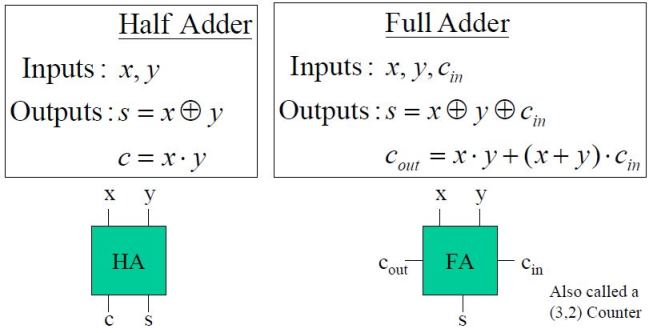
\includegraphics[width=0.7\linewidth]{img/img2/1}
\end{center}

where $a_i$ and $b_i$ are two incoming operands, $s_i$ is the output sum bit, $c_i$ and $c_{i+1}$ are input and output carry bits. Boolean equations describing full adder are:
\begin{eqnarray*}
s_i=a_i \oplus b_i \oplus c_i\\
c_{i+1}=a_i \cdot b_i+a_i \cdot  c_i+b_i \cdot c_i\\
\end{eqnarray*}

In terms of performance two time delay can be employed: $t_s$ is the delay between input and $s_i$, $t_c$ between input and carry out. Usually $t_s > t_c$ since the critical path is most of the time along carry propagation and so it is improved. With $t_{FA}$ we indicate the general delay of full adder (therefore assuming $t_c \approx t_s$).

\section{Ripple carry adder}
\begin{center}
  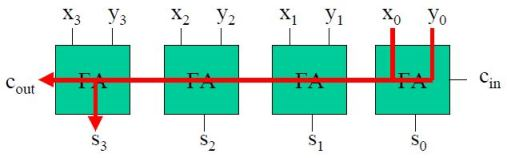
\includegraphics[width=0.7\linewidth]{img/img2/2}
\end{center}

Looking at this implementation complexity is linear with the number of bits, critical path is the one along carry out propagation. Assuming $t_s>t_c$ c.p. is the one along all carry out and going out from the last FA through its sum, so:

$$t_{cp}=(n-1)t_c+t_s$$

This architecture is modular and very simple, however its behavior in term of performance is not very nice since delay is proportional to the number of bit. A faster adder using this architecture cannot be build up.

\subsection{Bit serial}
\begin{center}
  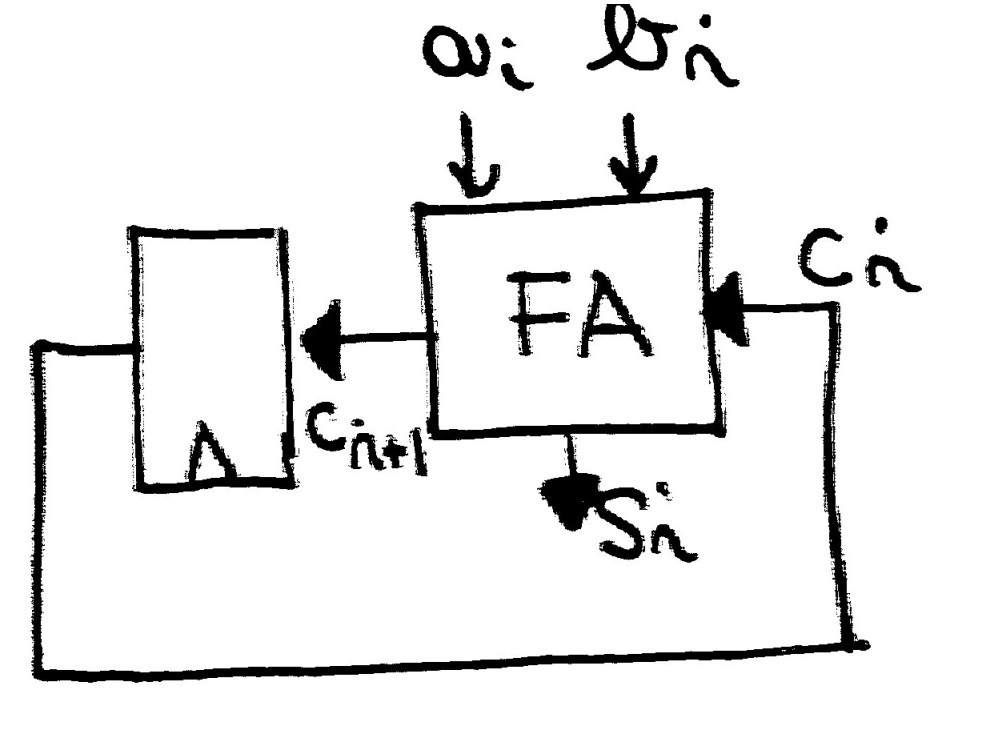
\includegraphics[width=0.5\linewidth]{img/img2/3}
\end{center}
It is the folded version of ripple carry adder (which is a parallel implementation). This is a nice example of decomposition: these last two implementations have different performance but the same ideal one. In the first architecture in a single clock cycle the information propagates n FA, while in the second n clock cycles are involved, meaning that parallel and serial have the same ideal throughput which is $\frac{1}{nt_{FA}}$.
Ideally performances are the same since we are neglecting delay along interconnects, delay introduced by registers and so on.
\section{Booth multiplier}

Starting from binary numbers they can be simplified by using a different representation. For instance if we have to compute  $15 \cdot A$, using a binary representation the coefficient 15 would be expressed uniquely as "001111". Let's suppose to have an internal extended alphabet made up of ${0,1,\overline{1}}$, now to represent 15 many possibilities exist:

\begin{center}
  \begin{tabular}{|c|c|c|c|c|c|c|c|}
    \hline
     & & & & & & Value & Required operations\\
    \hline
    0&  0&  1&  1&  1&  1&        $P=A+2A+4A+8A$&   3 additions\\
    0&  1&  0&  0&  0&  $\overline{1}$& $P=16A-A$&      1 difference\\
    \hline
  \end{tabular}
\end{center}

The advantages of using this representation allow to reduce a lot complexity in case we want to perform multiplication since it becomes just a series of sums properly shifted. This idea can be exploited to obtain adders based on this algorithm

\subsection{Booth algorithm}
Two consecutive digits are analyzed at the same time, in particular we notice that:
\begin{center}
\begin{tabular}{|c|c|c|c|}
  \hline
  $x_i$&  $x_{i+1}$&  What they represent&  Operation to be performed\\
  \hline
  0&    0&      in middle of sequence&  -\\
  1&    1&      in middle of sequence&  -\\
  1&    0&      Tail of sequence&   $-A \cdot 2^i$\\
  0&    1&      Head of sequence&   $+A \cdot 2^i$\\
  \hline
\end{tabular}
\end{center}
\subparagraph{Example}

Again we start from 15 whose binary representation is "00111". In LSB a dummy zero is inserted to recognize the tail of sequence of ones. We are shifting the window (| |) one position to the left by the time, windows of consecutive steps are overlapping.
\begin{center}
\begin{tabular}{|c|c|c|c|c|c|c|c|c|}
  \hline
  Step (i)& & & & & & & & Operation to be performed\\
  \hline
    0&    0&    0&  1&  1&  1&  |1& 0|&   $-A$\\
    1&    0&    0&  1&  1&  |1&  1|&  0&    nop\\
    2&    0&    0&  1&  |1&   1|&  1& 0&    nop\\
    3&    0&    0&  |1& 1|&   1&   1& 0&    nop\\
    1&    0&    |0& 1|& 1&    1&   1& 0&    $+A \cdot 2^4$\\
  \hline
\end{tabular}
\end{center}
Since in MSB positions we have only zeros no further operations have to be performed. Actually we can apply this algorithm also to numbers like "0010" resulting in $"01\overline{1}0"$. This is an interactive algorithm, so by looking at more than two-bit at the same time to speed up the executions. This approach leads to radix-4 version whose truth table is the following:
\begin{center}
\begin{tabular}{|c|c|c|c|c|}

\subsection{Flag}
Often we also need to generate some flags.

\subparagraph{Zero}
Zero flag ($z$) is asserted when every sum bit is equal to zero, so:
$$z=\overline{s_0+s_1+...+s_{n-1}} $$

\subparagraph{Overflow}

An overflow condition occurs when:
\begin{itemize}
  \item $a_{n-1}=b_{n-1}=0 \qquad s_{n-1}=1 $ (operands expressed in CA2 are positive and the result is negative).

  \item $a_{n-1}=b_{n-1}=1 \qquad s_{n-1}=0$ (operands are negative and the result is positive).
\end{itemize}

In both cases we can identify the overflow condition by:
$$o=c_n  \oplus c_{n-1} $$
i.e. xor between carry in and carry out of full adder in most significant position.

To justify this expression we notice that:
\begin{itemize}
  \item
    \subitem If $a_{n-1}=b_{n-1}$ then $s_{n-1}=c_{n-1}$.
    \subitem If $a_{n-1}=b_{n-1}=0$ then $c_n=0$.
  If overflow=1 then $s_{n-1}=1$ and $c_{n-1}=1$ therefore $c_n \oplus c_{n-1}=1$.

  \item
    \subitem If $a_{n-1}=b_{n-1}=1$ then $c_n=1$.
  If overflow=1 then $s_{n-1}=0$ and $c_{n-1}=0$ therefore $c_n \oplus c_{n-1}=1$.

\end{itemize}

\subparagraph{Sign bit}
Sign bit is computed as:

$$s=s_{n-1} xor o $$
meaning that if no overflow occurs sign bit equal to MSB bit, otherwise MSB has to be complement since the result is wrong. Even in case of overflow we are able to generate the correct sign bit.

\subsection{Carry generation}
Before looking at different architecture, we need to consider a different way to generate carry out.

\begin{center}
  \begin{tabular}{|c|c|c|c|c|}
    \hline
     $a_i$& $b_i$&    $c_i$&    $c_{i+1}$& Case\\
     \hline
      0&    0&    0&    0&    g\\
      0&    1&    0&    0&    a\\
      1&    0&    0&    0&    b\\
      1&    1&    0&    1&    e\\
      0&    0&    1&    0&    h\\
      0&    1&    1&    1&    c\\
      1&    0&    1&    1&    d\\
      1&    1&    1&    1&    f\\
    \hline
  \end{tabular}
\end{center}

Meaning that:

\begin{itemize}
  \item  In cases $a,b,c,d$ (i.e. $a_i$ different from $b_i$) then $c_{i+1}= c_i$, so we are in \textbf{propagate condition}, carry out has not to be computed.
  $$p_i=a_i \oplus b_i$$

  \item In cases $e,f$ carry out is asserted independently from carry in, there is no propagation but $c_{i+1}$ is set to one by the output sum bit of the adder, so it is a \textbf{generate condition}. This implies that if $a_i=b_i=1$ then $c_{i+1}=1$ and so:
  $$g_i=a_i \cdot b_i$$

  \item In cases $g, h$ output carry is always zero independently from the carry in, this is called \textbf{kill condition}. When $a_i=b_i=0$ then $c_{i+1}=0$ and so:
  $$k_i=\overline{a_i+b_i}$$

\end{itemize}

Using $p_i, g_i, k_i$ it is possible to compute carry out bit.

\section{Carry skip adder (CSKA)}

\begin{center}
  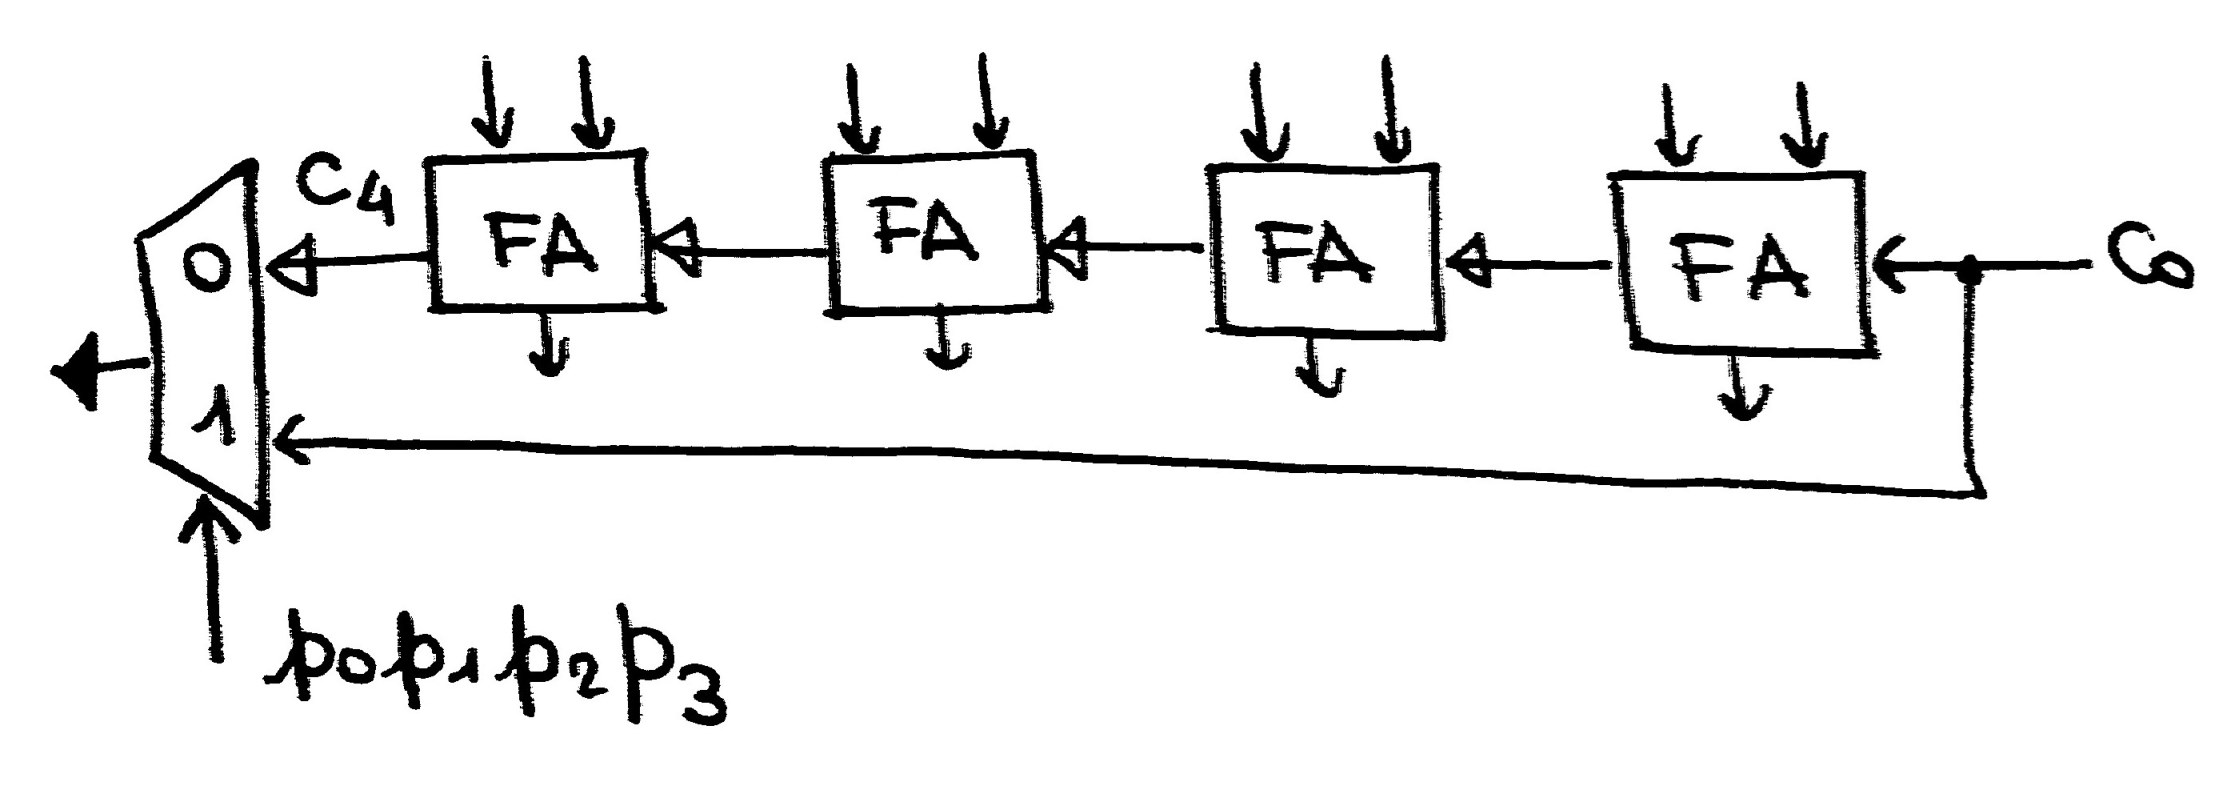
\includegraphics[width=0.7\linewidth]{img/img2/4}
\end{center}


Starting from RCA let's imagine to allocate also some additional gates to calculate propagate bits for each stages. If $p_0=1$ it means that $c_1$ is equal to $c_0$, then if $p_1=1$ also $c_2$ will be equal to $c_1$; therefore if all $p_i$ are equal to one the carry in propagates from input to output. This is actually a particular case but it corresponds also to the worst one for delay, in fact the situation for which the overall propagation of the carries takes place corresponds to critical path and is therefore very important.\\

Summarizing if $p_0\cdot p_1 \cdot p_2 \cdot p_3=1$ we can anticipate the carry, otherwise it has to be computed. In any case, also if $p_0=0$ it means that in stage 0 there will be a generate or a kill, so in both cases the critical path has been reduced since it does not start from $c_0$ but from $b_0$ or $a_0$. CSKA is faster only if we have the overall propagation, otherwise the delay is a little bit greater due to multiplexer.

By applying this idea to a buffer adder:

\begin{center}
  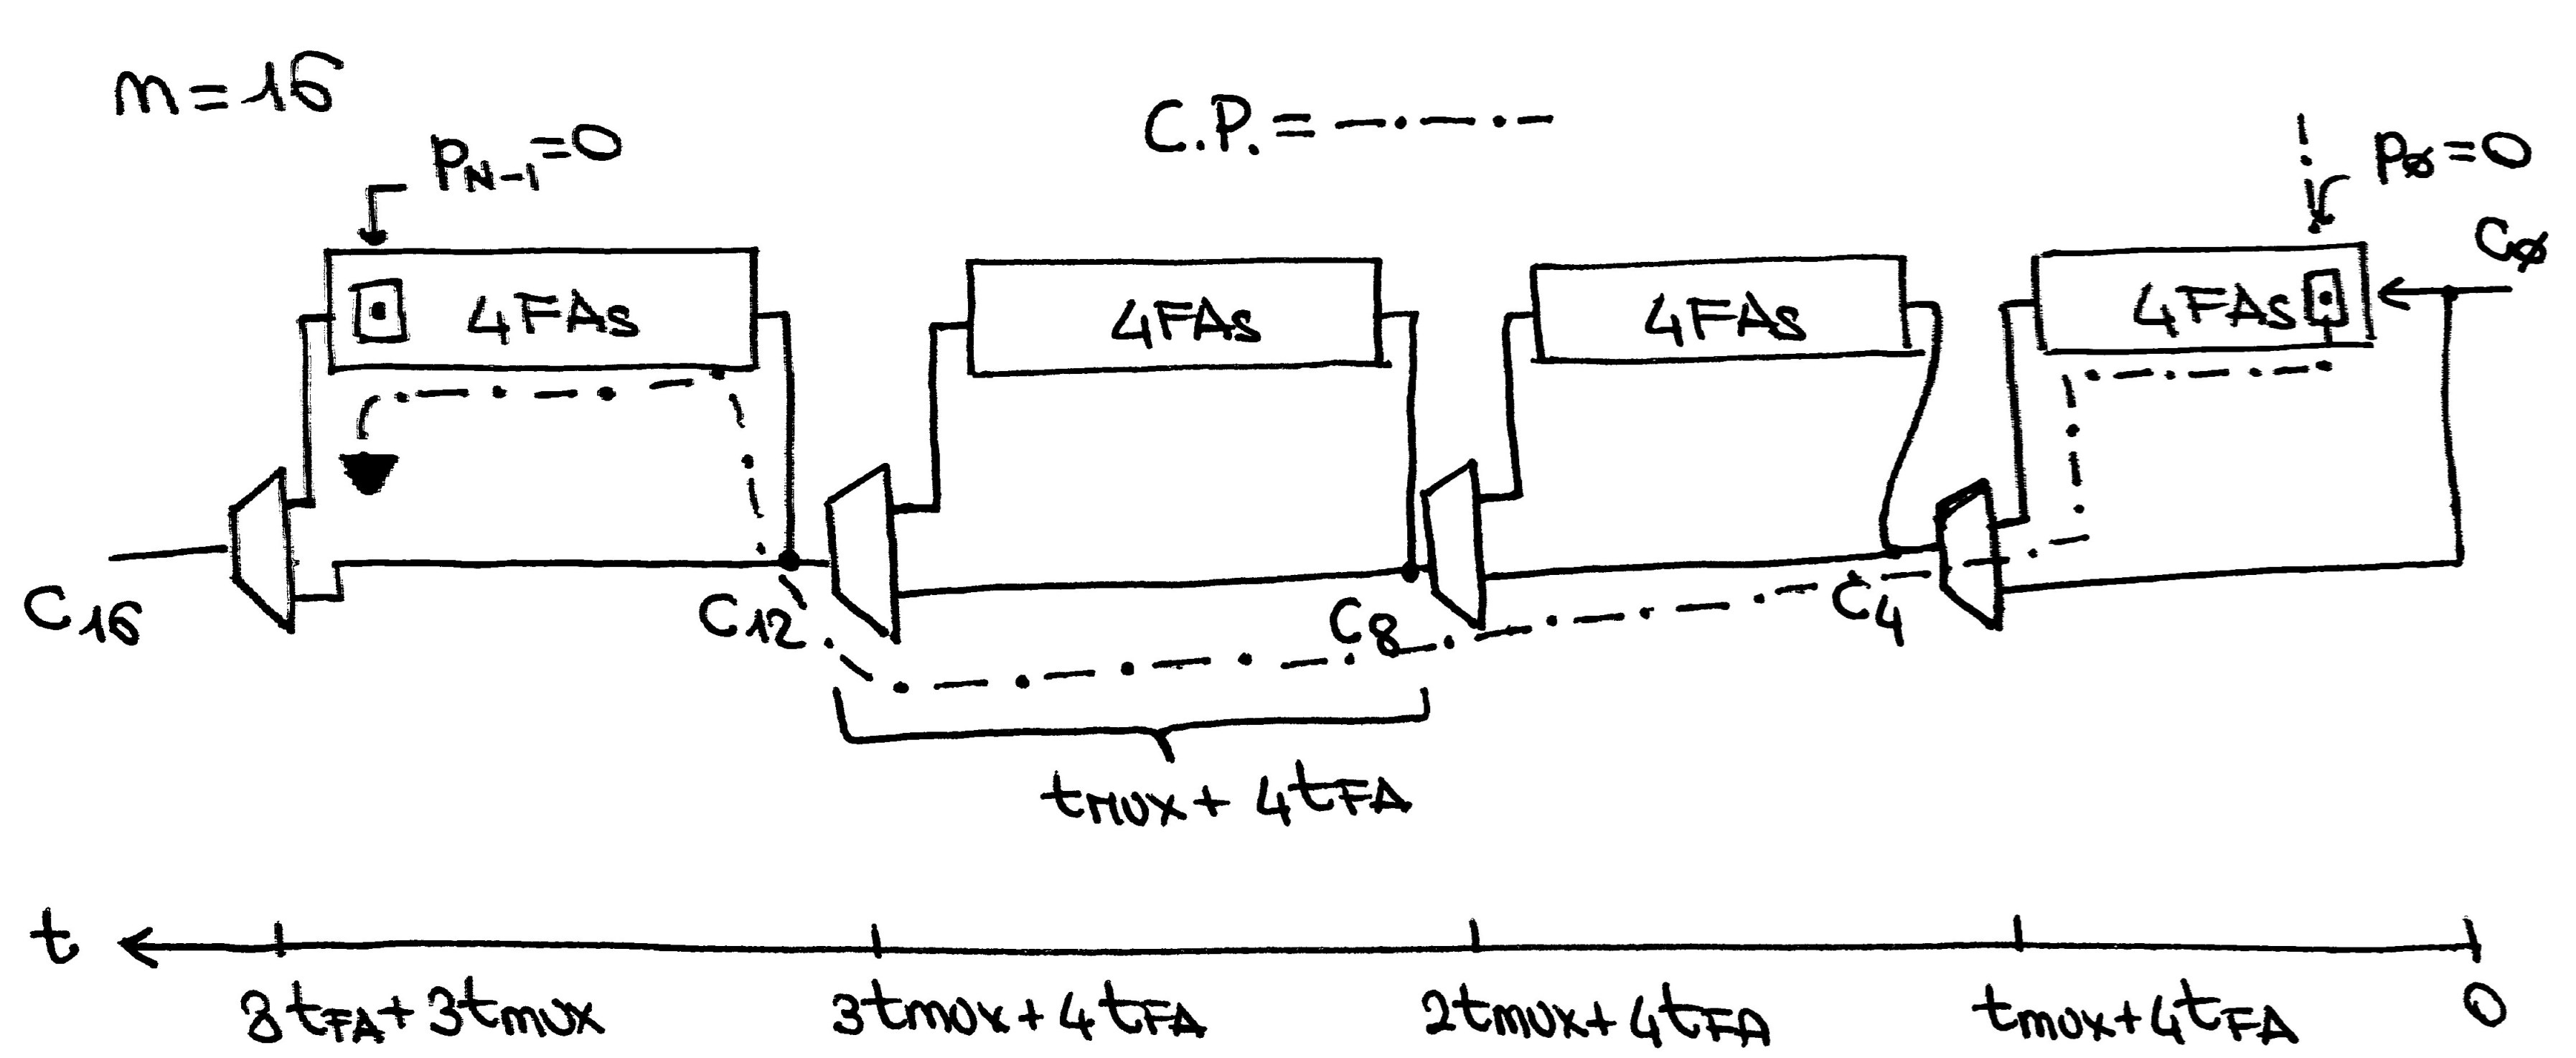
\includegraphics[width=0.8\linewidth]{img/img2/5}
\end{center}


Critical path is the one for which $p_0=0, p_1=p_2=p_3=1$ since any other combination of $p_i$ leads to a shortest delay. Across the second block instead the worst case is when all $p_i =1$, same thing occurs for block 3 and so on. Regarding the last block if all $p_i=1$ then we will skip these adders and just take the multiplexer delay, but if $p_{n-1}=0$ our carry will propagate up to the last FA and then stop here so we have to pass through all FA of last adder.

At the MSB global delay is $t_d=8t_{FA}+3t_{mux}$.

In general for a $n$ bits adders, made up of $b$ blocks with $k$ bits each (so $n=k \cdot b$), global delay can be expressed as:
$$t= (b-1)t_{mux} + 2 *k* t_{FA}= (b-1)t_{mux} + 2 \cdot \frac{n}{b} \cdot t_{FA}$$

Critical path goes through first and last blocks while in intermediate blocks carry is always propagated (in this way we don't break the propagation from input to output and don't consider a shortest critical path).\\
Taking the derivative of final expression and by setting it equal to zero, the optimal number of blocks is the one for which:

$$b_{opt}=\sqrt{\frac{2nt_{fa}}{t_{mux}}}$$

Corresponding to optimal delay:

$$t_{min}=\sqrt{2nt_{TA}t_{mux}}-t_{mux}+2nt_{FA} \sqrt{\frac{t_{mux}}{2nt_{fa}}}$$

By the way $b_{opt}$ must be an integer number.

Delay is proportional to $\sqrt{n}$ so the behavior is not linear like RCA and growing speed is much slower than previous architecture.\\

Some additional improvements to CSKA can be performed by assuming to have defined an optimal number for $b$. Minimizing $k$ is useful to reduce the second delay contribution while reducing $b$ we can reduce the first term; but unfortunately we cannot modify independently $k$ and $b$ because they are related. If we image that every block may have a different number of FA we are introducing a freedom degree. The idea is that internal blocks are bigger than starting and lasting one, so we can reduce $k_0t_{FA}$ and since the internal $k_j$ are bigger there will be less blocks leading to a smaller delay associated to multiplexers.
\begin{center}
  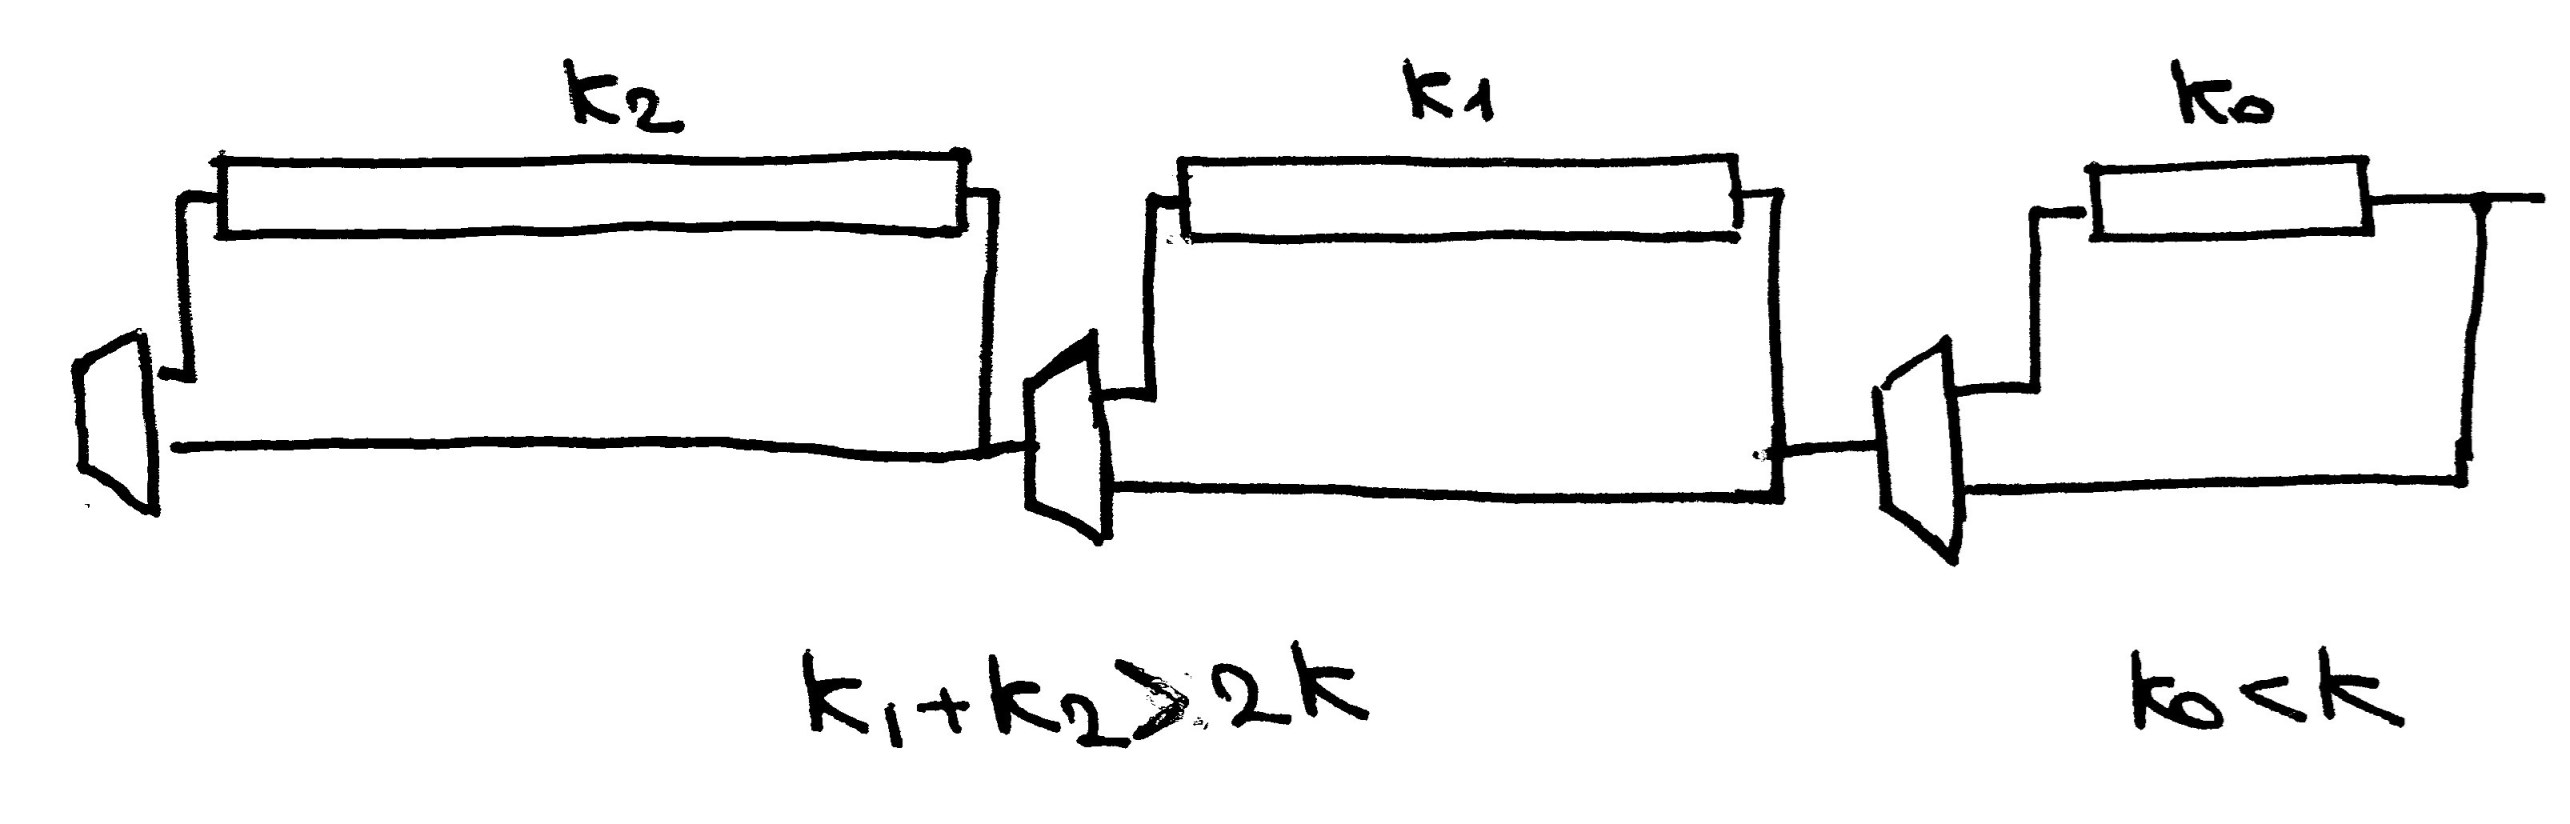
\includegraphics[width=0.7\linewidth]{img/img2/6}
\end{center}


Delay is still proportional to $\sqrt{n}$ but the coefficient is smaller than before, the idea of skipping blocks can be further exploited improving coefficient but not the kind of function.

 \section{Carry select adder (CSA)}
 In this architecture a brute force approach is employed since we try to stop the complete propagation of carry. Starting from a 4 bits RCA and by putting another 4 bits RCA for the second block, we must to wait the propagation of carry along the first RCA. Since we want to avoid it, for the second block we allocate two identical blocks, where for one of them we assume that $c_{in}=0$ and for the other one that $c_{in}=1$, in this way there are 3 RCA working in parallel. The idea is to allocate additional adders to compute all possible cases and then choose the correct one.

\begin{center}
  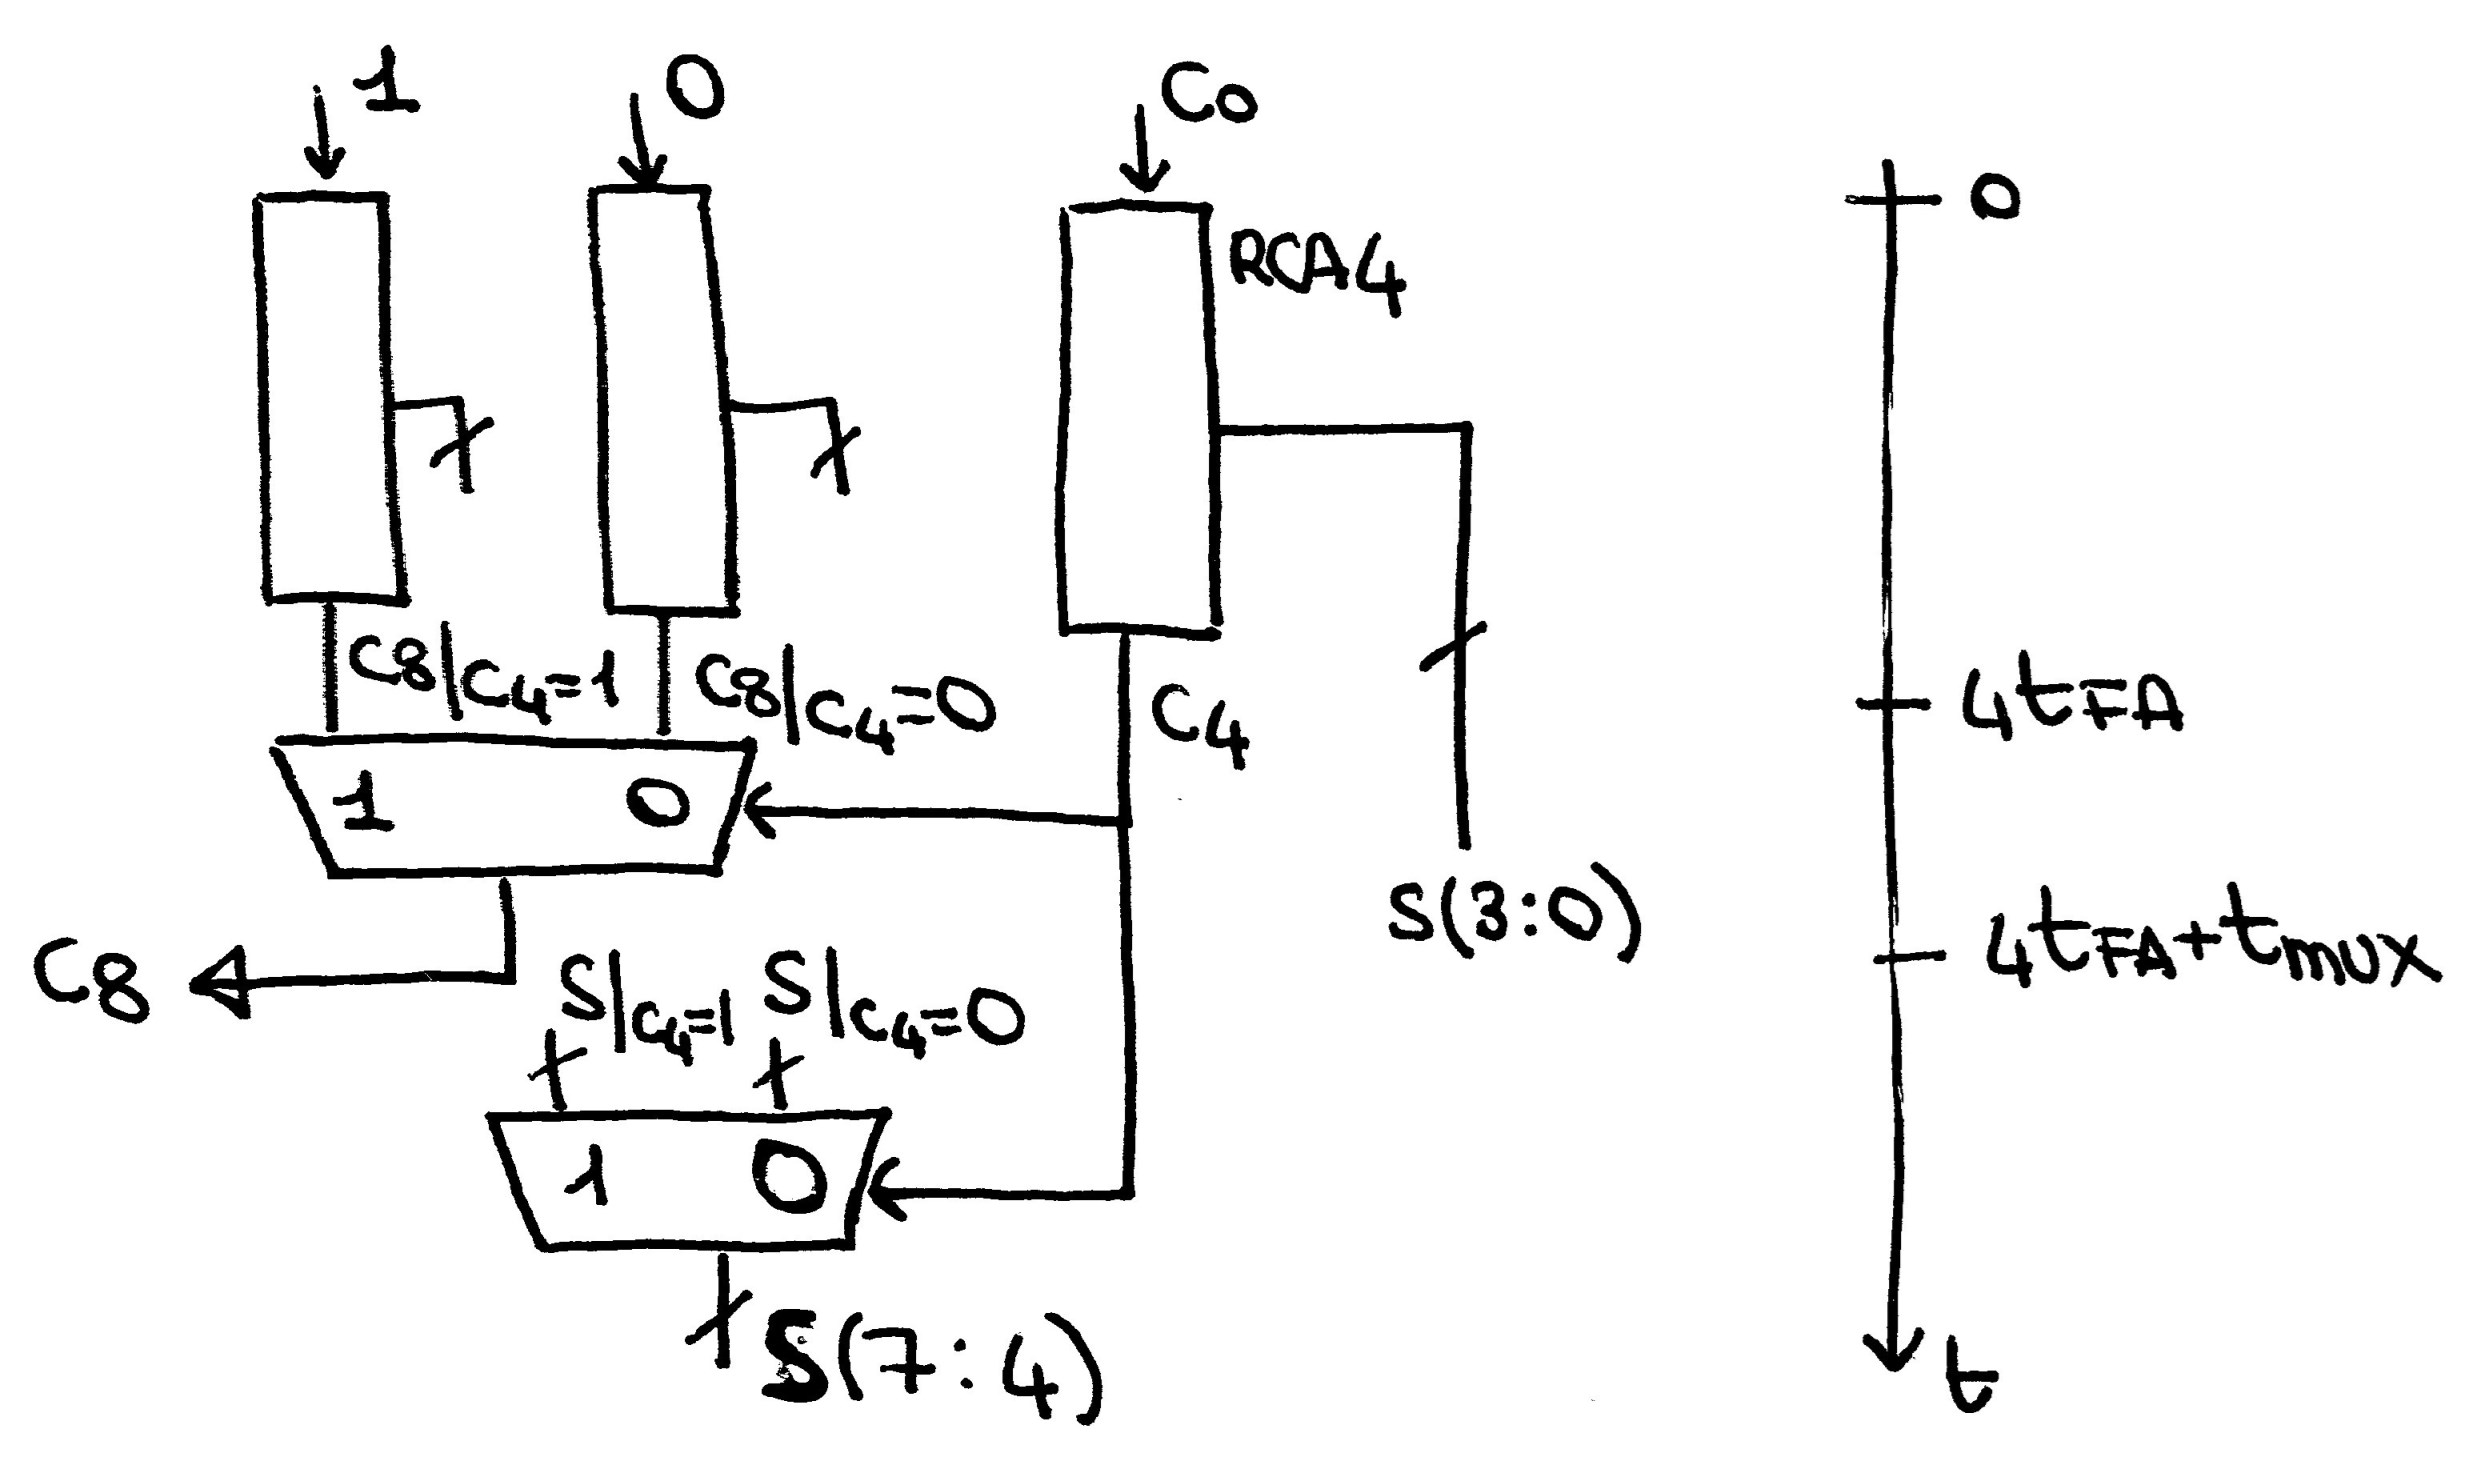
\includegraphics[width=0.7\linewidth]{img/img2/7}
\end{center}


 Two different architectures can implement this idea in a real full adder.

 \subsection{Linear approach}

Assuming n=16, k=4 bits/blocks

\begin{center}
  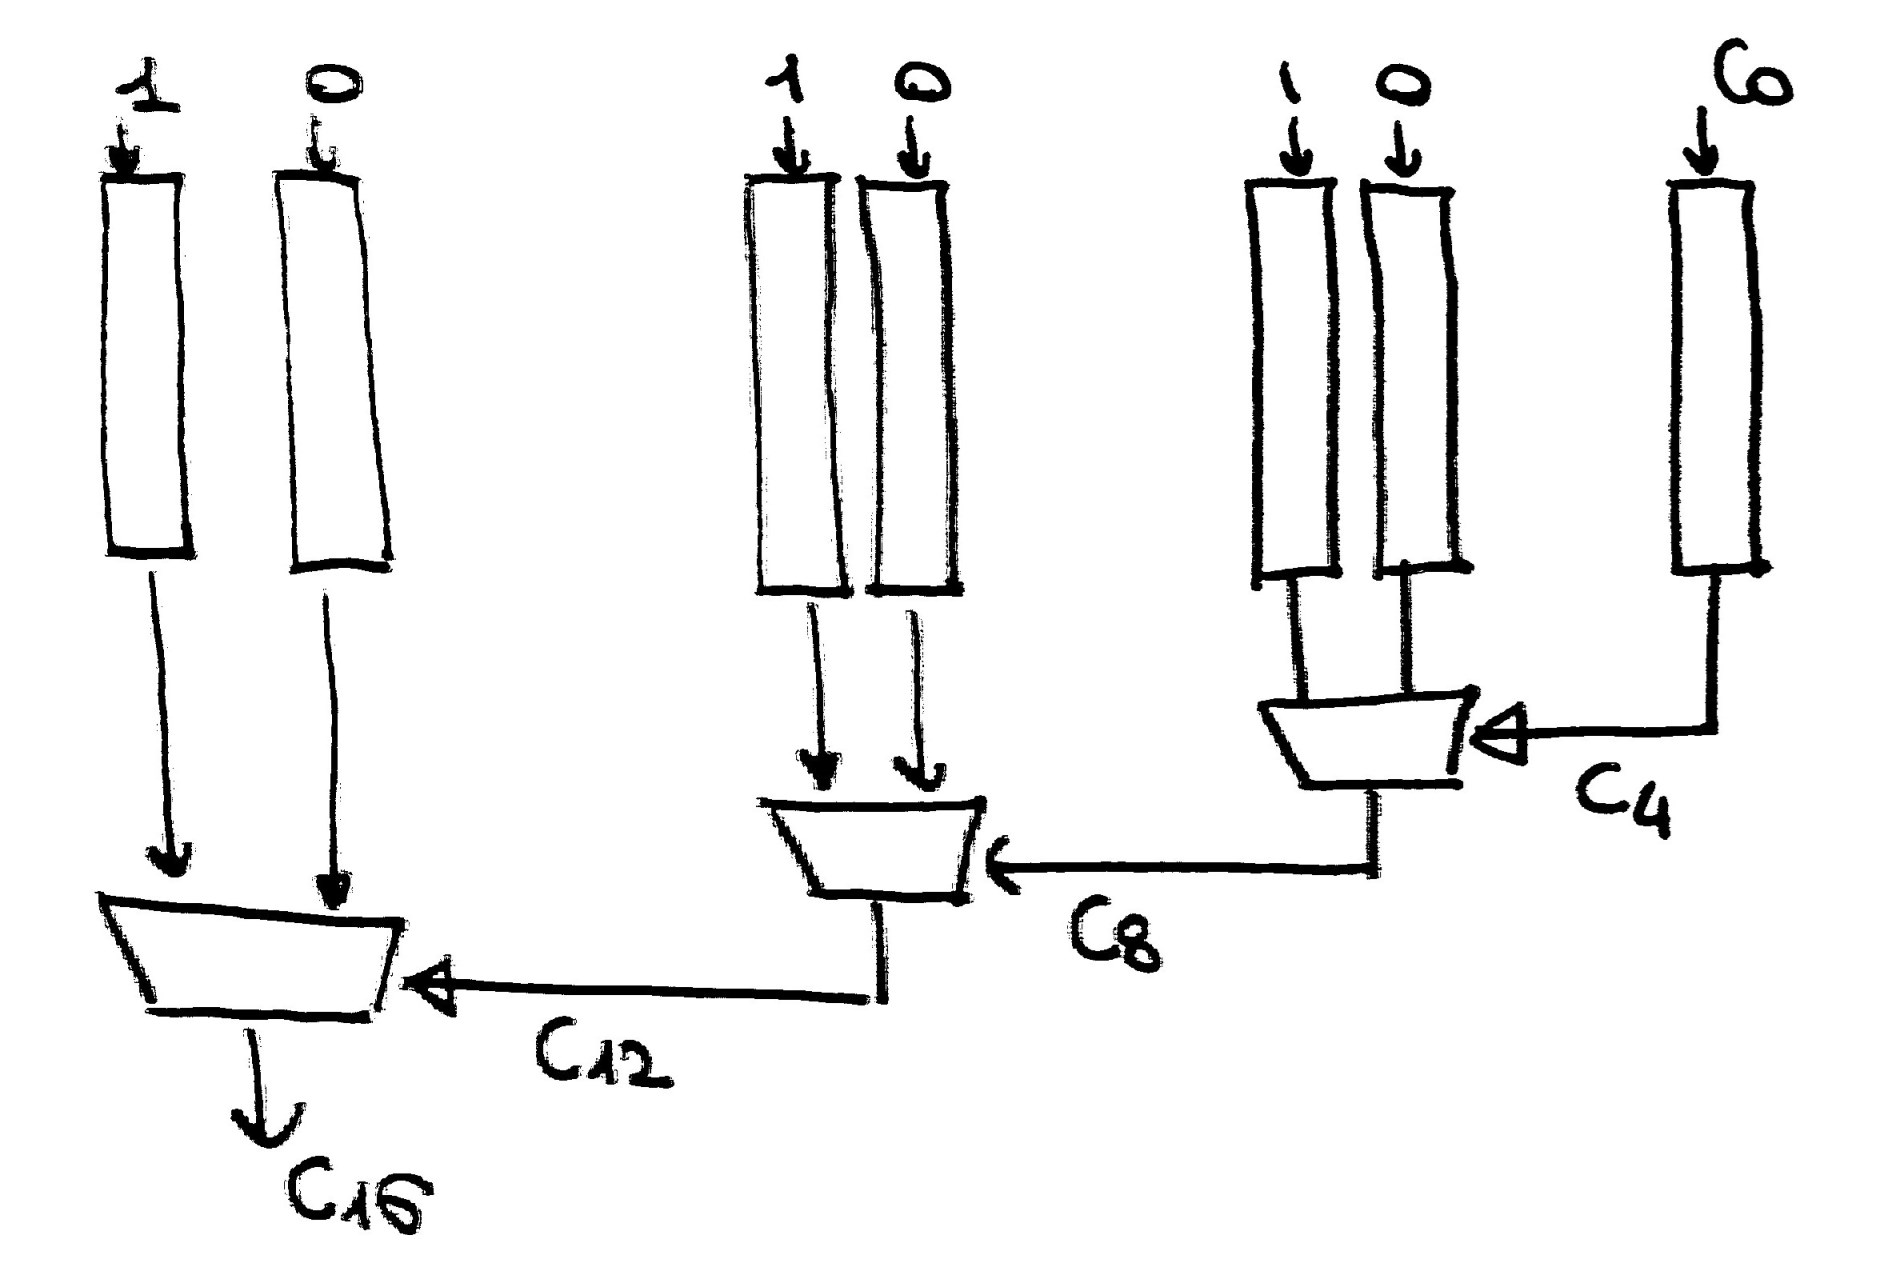
\includegraphics[width=0.7\linewidth]{img/img2/8}
\end{center}

 We allocate two RCA-4 bit for each block/stage acting in parallel. This is a linear approach since the delay increases linearly with the number of multiplexer.
 With $n=16$ the global delay is $t_d=4t_{fa}+3t_{mux}$. For a generic $n$ bits adder made up of $b$ blocks with $k$ bits/blocks, the total delay is:

 $$t=kt_{fa}+(b-1)t_{mux}$$

Since $b=n/k$ we can derive wrt $k$ to find the optimal solution:

$$t=kt_{fa}+(\frac{n}{k}-1)t_{mux}$$

By fixing $n$ and optimizing with respect to $k$:

$$ \frac{\partial t}{\partial k} = 0 \longrightarrow  t_{fa}- \frac{n}{k^2} t_{mux}=0 \longleftrightarrow k=\sqrt{\frac{nt_{mux}}{t_FA}} $$

By choosing the proper $k$ we can reach same performance of skip carry adder but with double area so it not a very big improvement.\\

In this architecture every block works in parallel and complete its task at the same time of the other ones but then we have to wait for three multiplexer: we can accept that blocks have not the same length since for instance in the last one we have to wait the propagation of the carry in the previous multiplexers, so the starting block will be the shortest while the last one the longest. In this way we obtain a smaller coefficient but the dependency is always sub-linear.

\subsection{Logarithmic approach}
To obtain a logarithmic law a binary tree organization is required, so assuming that $N$ is equal to the adder parallelism, initially we divide N into two equal parts $(0 \rightarrow \frac{N}{2}+1) (\frac{N}{2} \rightarrow N-1)$, for the lowest part we allocate just one block while for the second we allocate two equal blocks working in parallel. Then we proceed in the same way by dividing one of this three block and reusing carry select approach, so for the least significant block we apply exactly the same scheme (same topology, only indexes change). Same thing occurs for most significant bits since we can split into N/4 bits blocks. Carry out it's determine by $c_{\frac{3n}{4}}$ so we need to allocate two multiplexers having same inputs but different selecting signal.

\begin{center}
  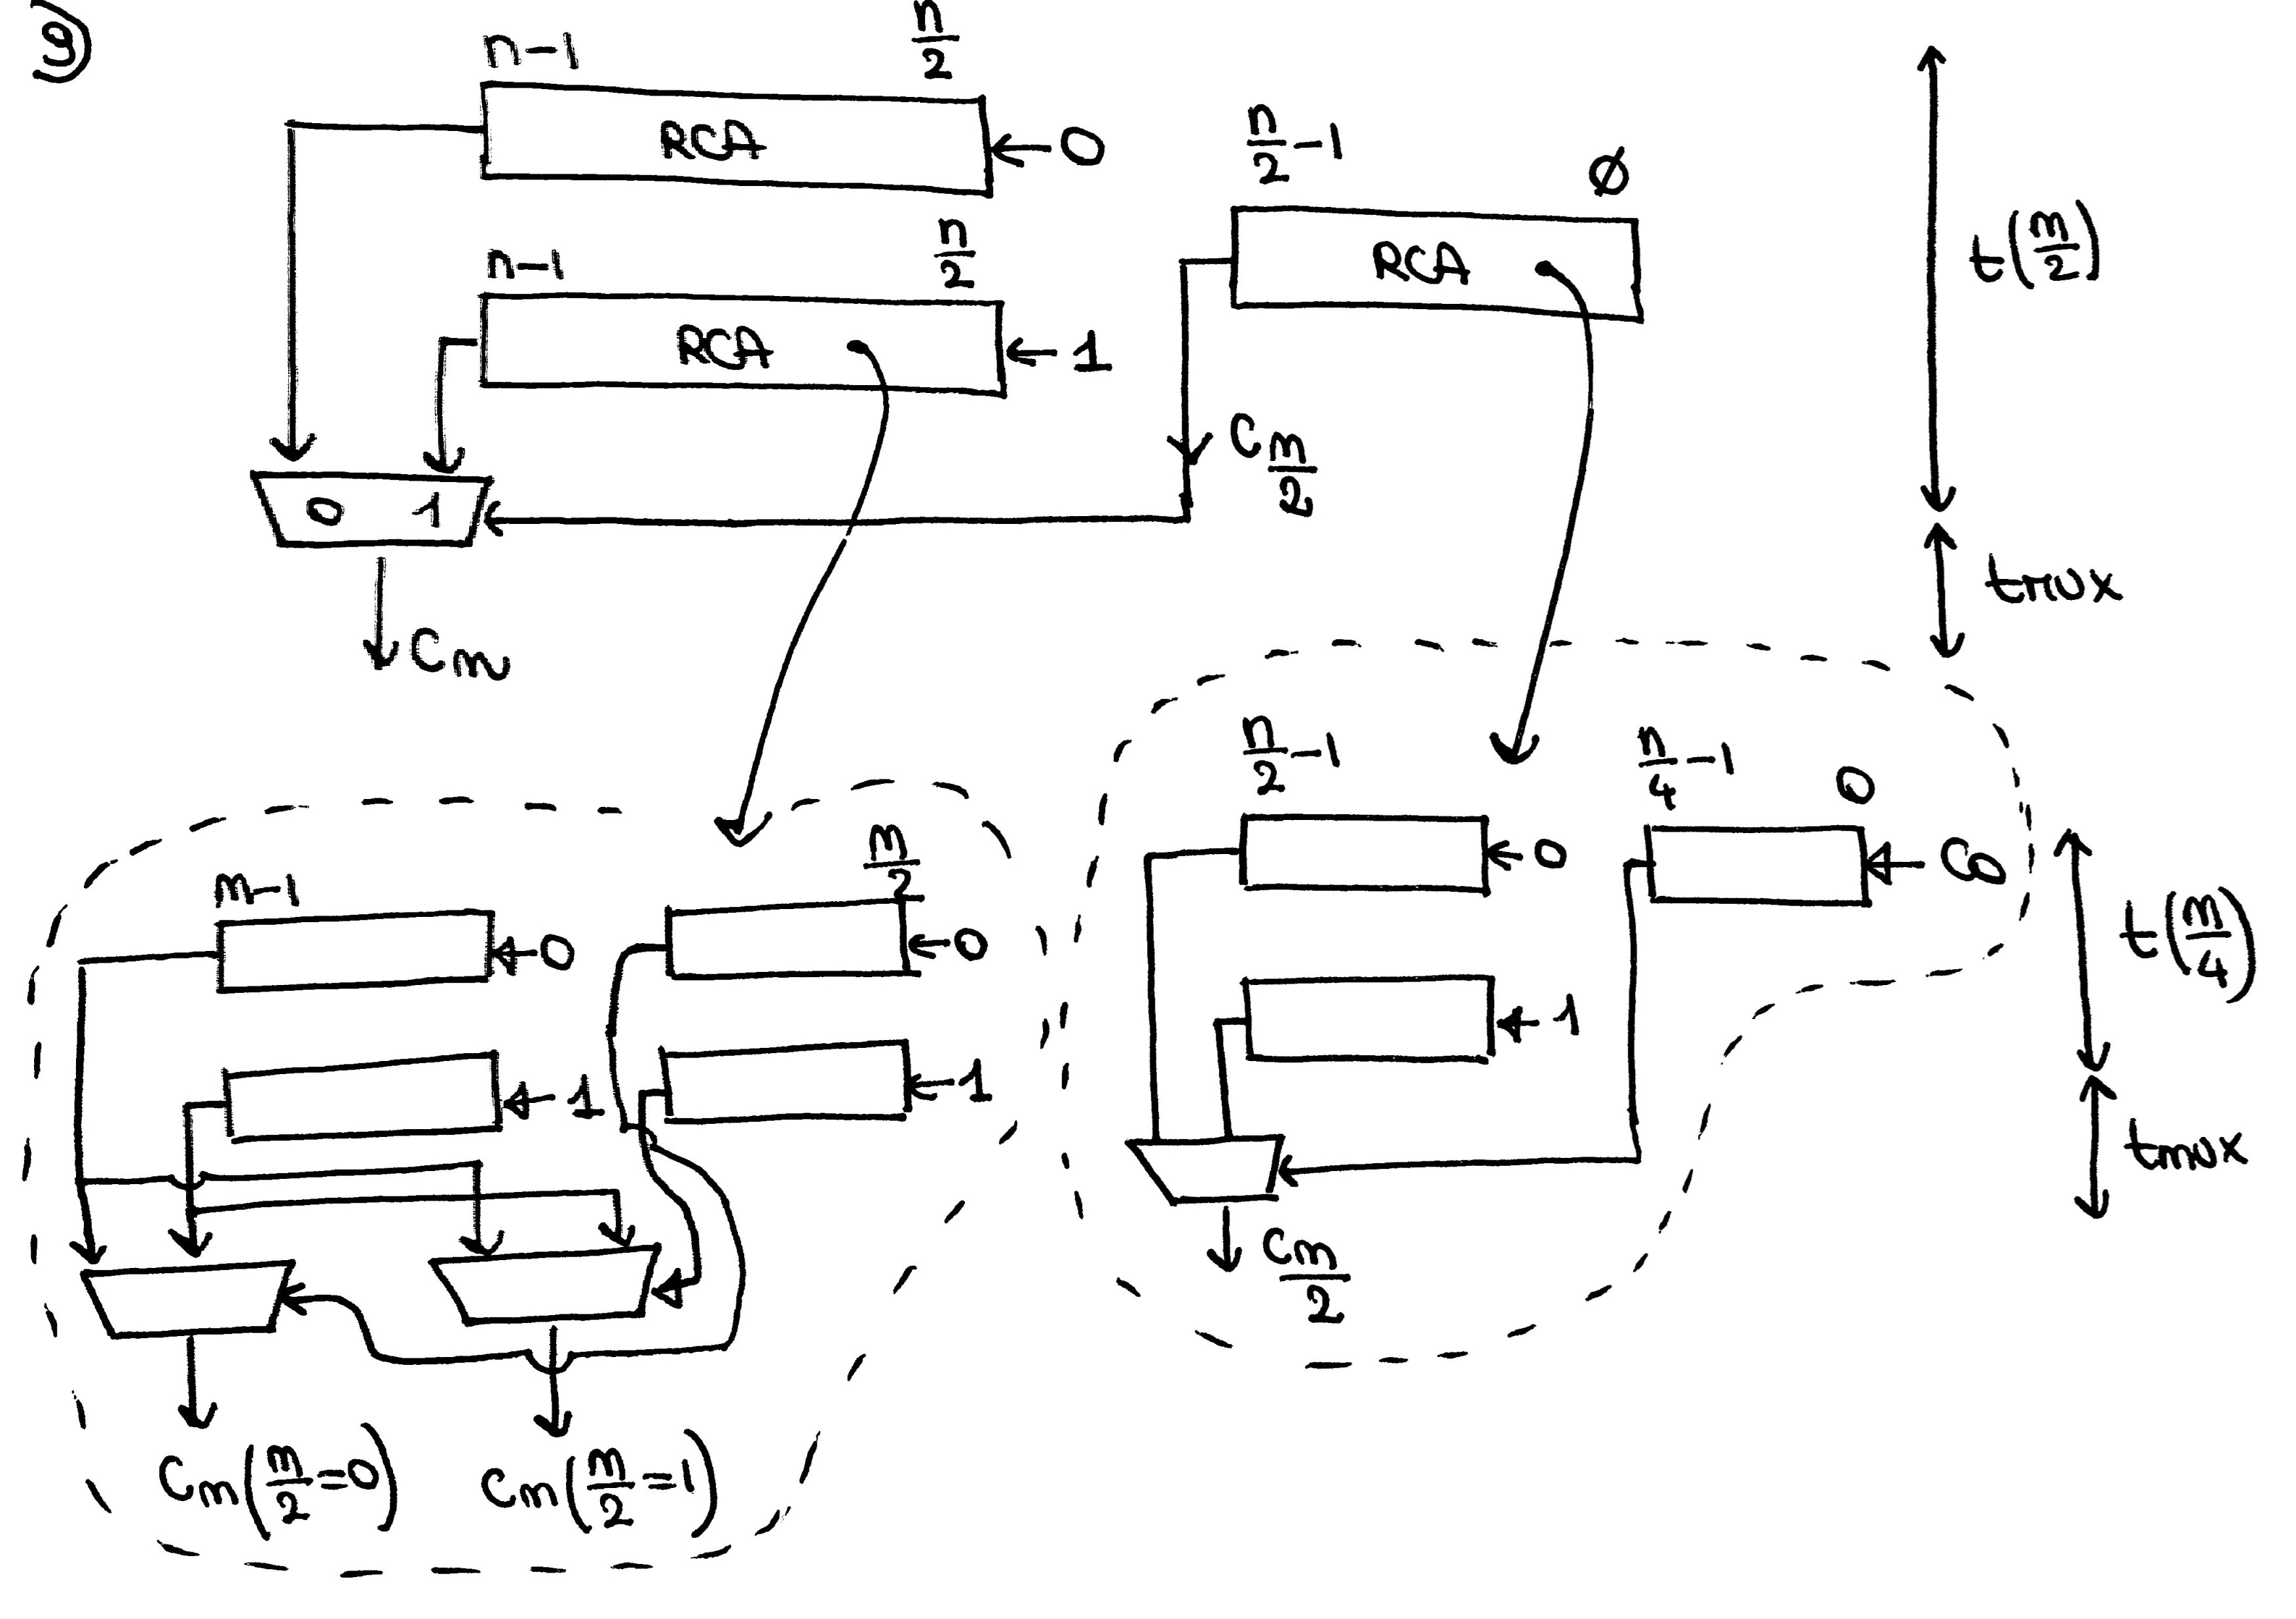
\includegraphics[width=0.7\linewidth]{img/img2/9}
\end{center}


Every time we perform this decomposition we add a new multiplexer layer. Applying this approach more than one time:

\begin{center}
  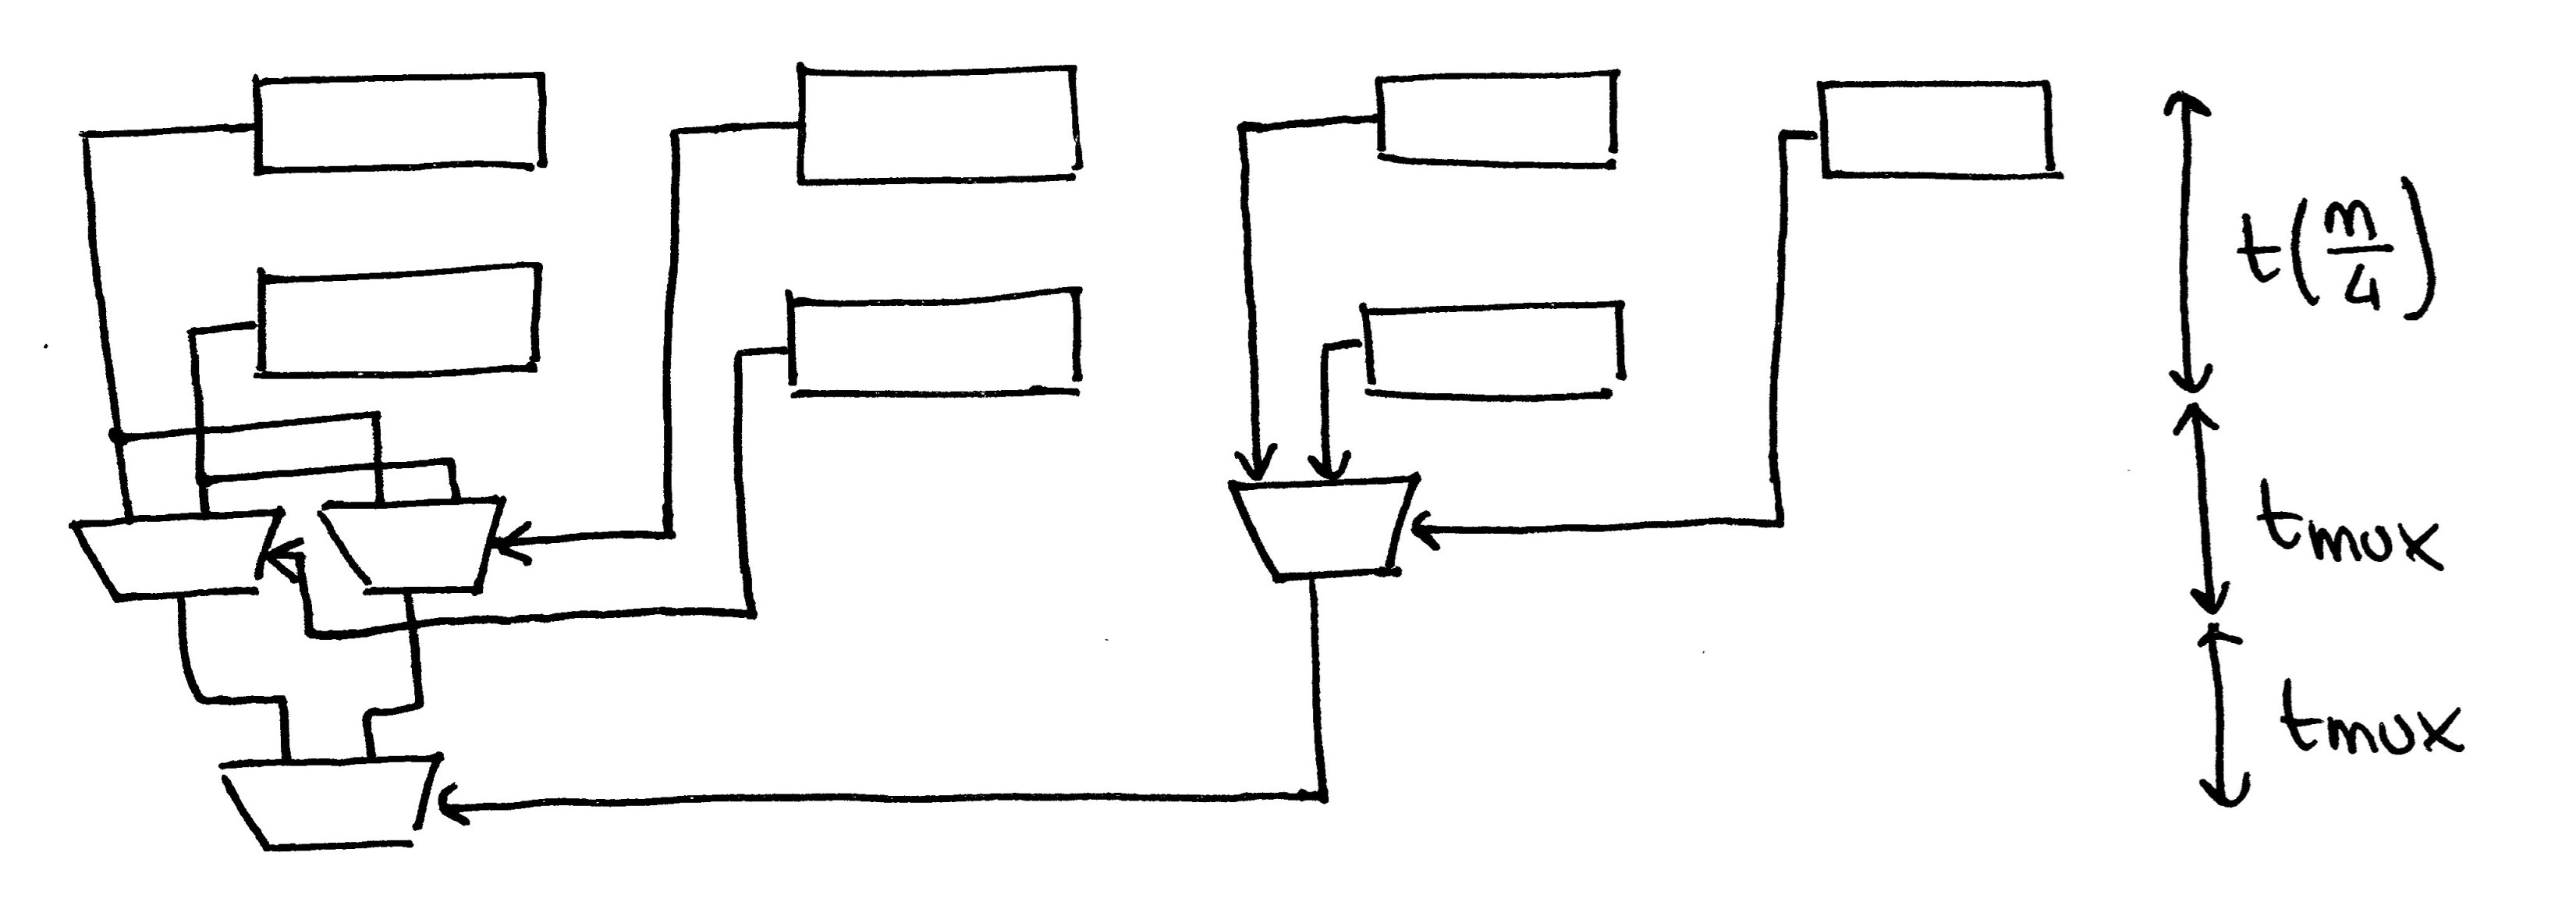
\includegraphics[width=0.7\linewidth]{img/img2/10}
\end{center}


By calling $k$ the amount of decomposition adopted, $k$ is also equal to multiplexer levels, the delay of each level can be expressed as:

\begin{center}
\begin{tabular}{|c|c|}
  \hline
  $t(N/2)+t_{mux}$&     $1^{st}$ level\\
  $t(N/4)+2t_{mux}$&    $2^{nd}$ level\\
  $t(N/8)+3t_{mux}$&    $3^{rd}$ level\\
  $t(N/2^i)+it_{mux}$&  $i^{th}$ level\\
  \hline
\end{tabular}
\end{center}

Decomposition can be exploited up the point where each block is a single full adder (working on just one bit), at this point $t_{FA}=t(1)=t(n/2^h)$  where $n=2^h \rightarrow h=log_2 n$
and so the total amount can be written as:

$$t(n)=t_{fa}+log_2(n) t_{mux}$$

\subparagraph{Example: 16-bit adder}

In this case first three blocks are working on two bit each. In terms of speed it's very powerful but we need to allocate 2x full adders and multiplexer, so we are looking for other solutions. One of the most popular is the carry look-ahead adder.

\section{Carry look-ahead adder}
 Recalling generate and propagate bit:

 \begin{eqnarray*}
 g_i=a_i \cdot b_i\\
 p_i=a_i \oplus b_i\\
 c_{i+1}=g_i+p_i \cdot c_i\\
 \end{eqnarray*}

Output carry is asserted either if the input carry is equal to one and we are in propagate either if we are in generate (independently from input carry). Last expression can be simplified by computing $p_i=a_i + b_i$ (OR instead of XOR) then $c_{i+1}=g_i+p_i c_i$ is still valid but the meaning of propagate has been lost, so if $p_i$ is equal to one it's no more true that surely carry out equal to carry in, it may be or not. The only difference occurs when $a_i=b_i=1$, so $p_i \cdot c_i$ may be different but $g_i$ is guarantee to be equal to one. So there is no reason to use xor, we will use a simpler or (easier implementation) however it's no more correct call this signal propagate.\\

In principle every level of carry can be obtained by two-level logic:

\begin{center}
  \begin{tabular}{|c|c|l|}
    \hline
    Level& Carry out& Expression\\
    \hline
     0&   $c_0$&  \\
    1&    $c_1$& $g_0+p_0c_0$\\
    2&    $c_2$& $g_1+p_1c_1=g_1+p_1(g_0+p_0c_0)=g_1+p_1g_0+p_1p_0c_0$\\
    3&    $c_3$& $g_2+p_2g_1+p_2p_1g_0+p_2p_1p_0c_0$\\
    \hline
  \end{tabular}
\end{center}

Apparently at any level the delay is the one of two gates however in CMOS logic a 4-input OR is not so fast. Since at each further level there will be one more input this implementation can be applied up to 4-5 level. Organizing a little bit better the computing of generate/propagate we can obtain some improvements.\\

Looking at $g_i$ it's a 1 bit signal which is asserted if we expect to have $c_{i+1}=1$ because it's generated by full adder in position $i$. Instead a working on a single bit we define a block generate signal which is high if the carry is generated inside that block. Formally we call:

\begin{itemize}
  \item \textbf{Block propagate}: the notation $P_{0,1}=p_0p_1$ corresponds to consider {0,1} as range, inside which there is a propagation from input of FA 0 to output of FA 1 if both full adders are in propagate condition.
  \item \textbf{Block generate}: the notation $G_{0,1}=g_1+g_0 \cdot p_1$ corresponds to the condition in which there is a generation in FA1 or generation in FA0 and propagation in FA1.
\end{itemize}

\begin{center}
  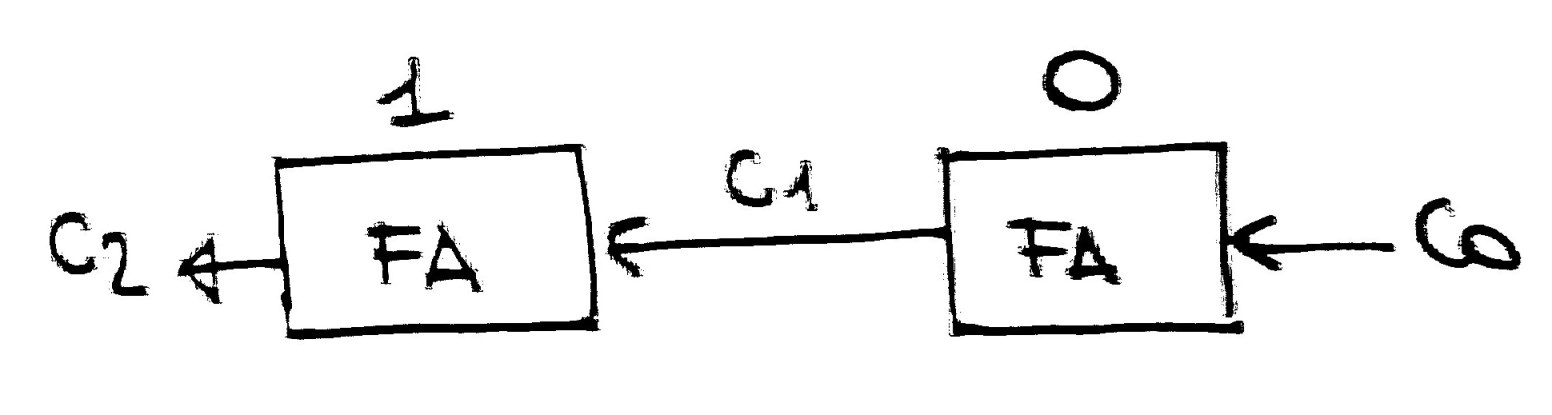
\includegraphics[width=0.6\linewidth]{img/img2/11}
\end{center}


These definitions can be applied to any level block where block size is arbitrary. In general it is possible to write:
$$P_{i,j}=p_ip_{i+1}p_{i+2}..p_{j}$$
$$G_{i,j}=g_j+g_{j-1}p_j+g_{j-2}p_{j-1}p_j$$

A very useful situation is when we have to compute carry out for a block which has been subdivided, meaning that starting from range (i, j) we split it into (i, k-1) and (k, j) (assuming j greater than i), in this case we can write:

$$P_{i,j}=P_{i, k-1} \cdot P_{k, j}$$
$$ G_{i, j}=G_{k, j}+G_{i, k-1}\cdot P_{k, j}$$

These new propagate/generate representations can be exploited to implement a tree-like topology capable of obtaining a logarithmic dependency of the delay in function of N.\\

Defining the following basic blocks:

\begin{center}
  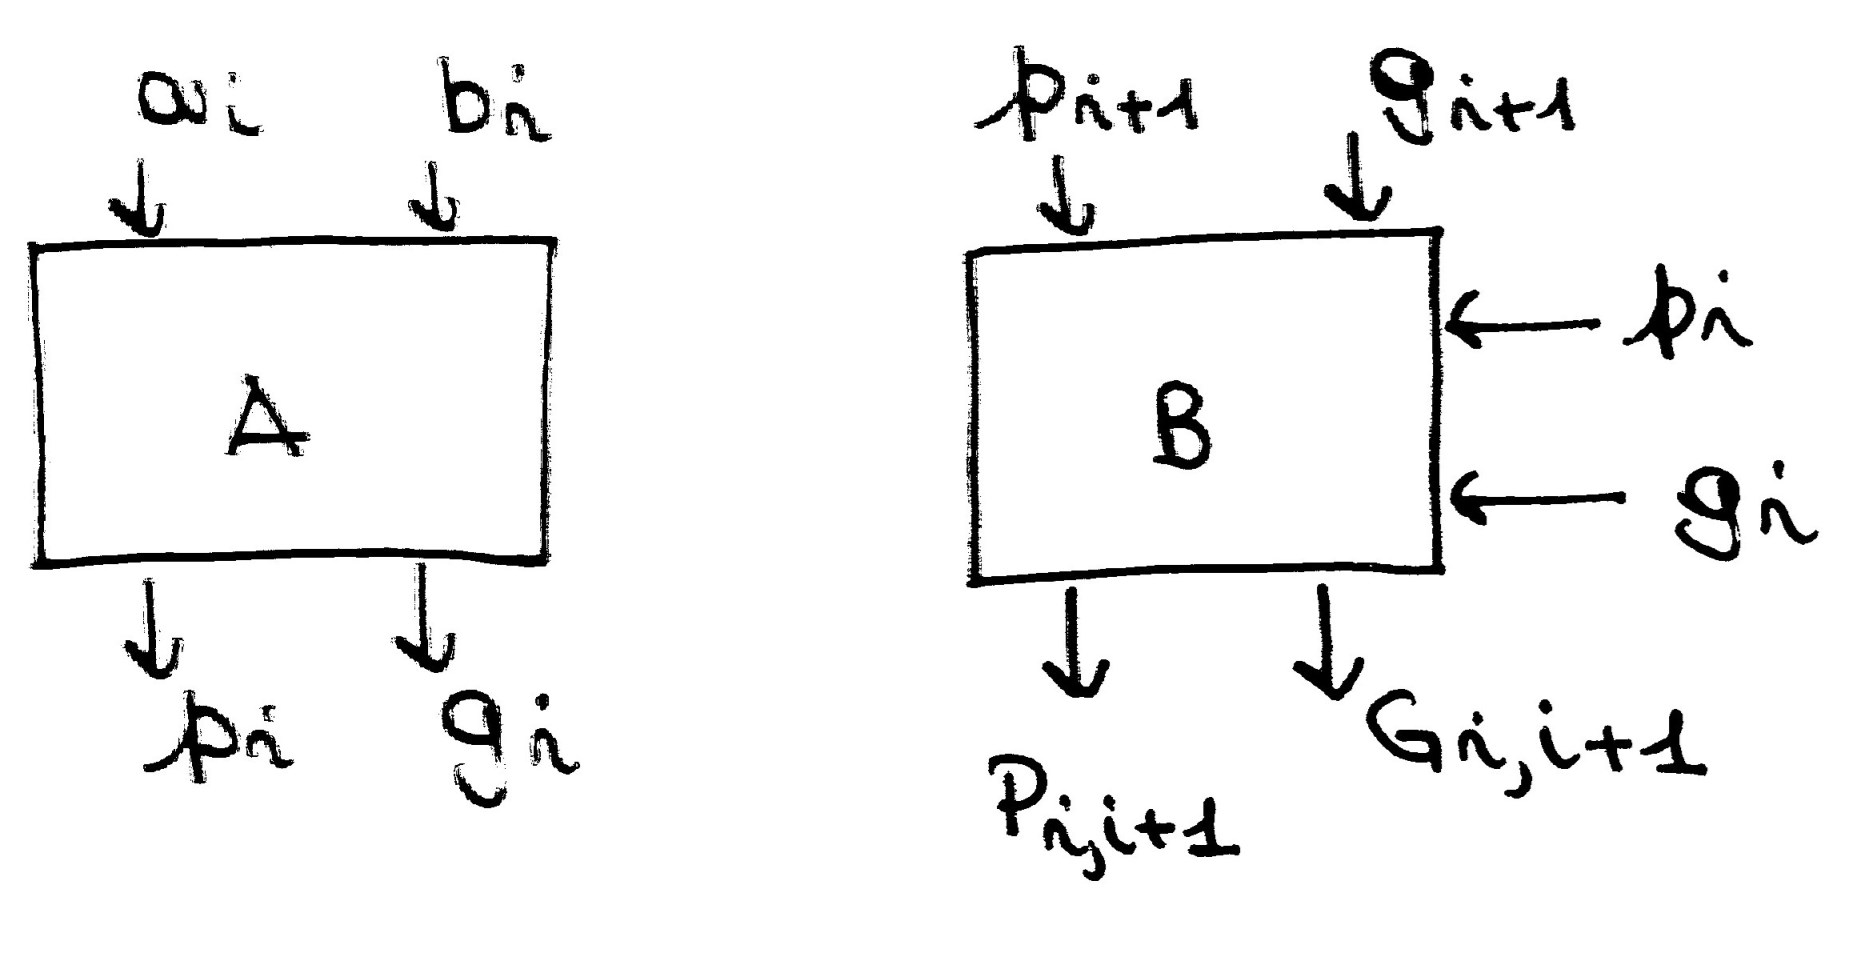
\includegraphics[width=0.6\linewidth]{img/img2/12}
\end{center}

By using them we can organized the addition in the following way:

 $\#$fig 13 (solo matita)

In first level propagate and generate are the classic bits, in second level using block B we are mixing two 2 propagate/generate and generating at the output 4 signal blocks.

We are building up a tree system where range length is doubled at each level. The key difference with respect to long boolean equations is in the use of block system, in this way we don't have to pass through a linear structure but through a logarithmic one. If we have to pass from 8 to 16 or 16 to 32 bit adders we just have to add one more level (no double of critical path). However we still have to compute $c_7$, to perform this the functionality of block A is extended so we suppose that starting from a $c_i$, it can also compute $s_i$. Moreover also B block must be slightly modified:
\begin{center}
  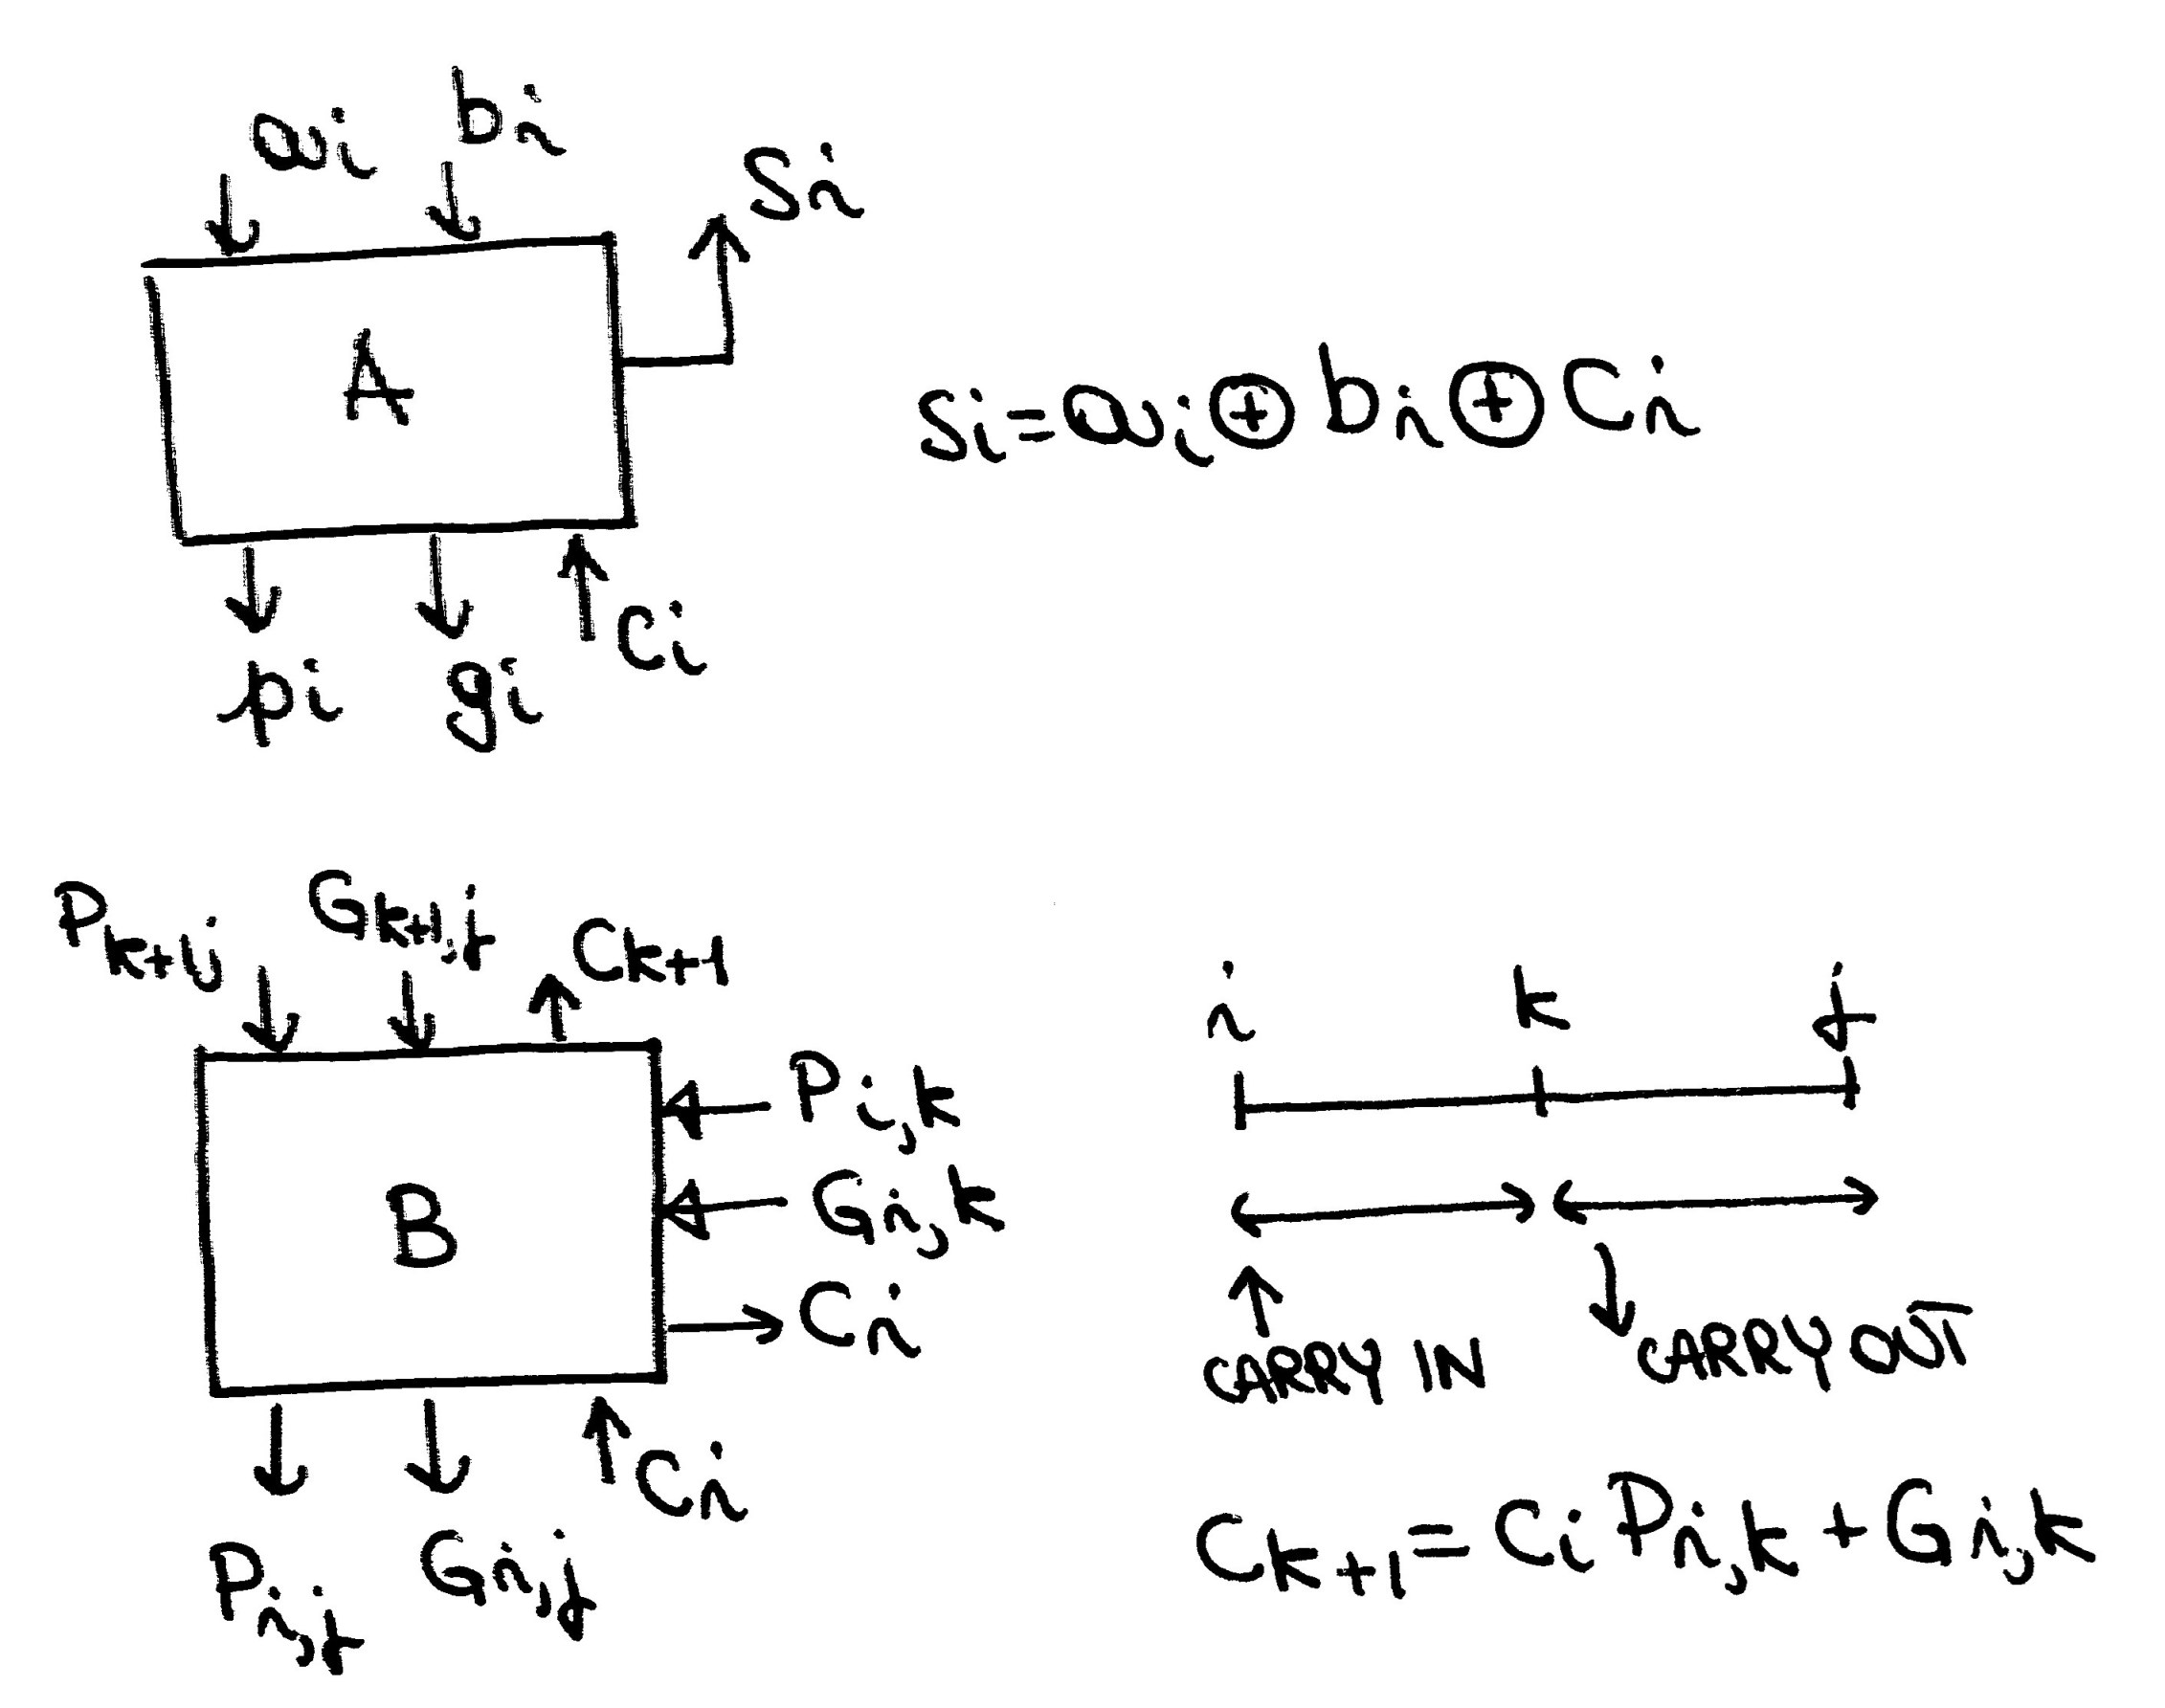
\includegraphics[width=0.6\linewidth]{img/img2/14}
\end{center}

B block is implementing two tasks: from top to bottom are the original equations, from bottom to top it generates the carry out in the least significant part.

If we modify the previous scheme using this extended blocks, we obtain:
\#fig 13 a colori

We have the possibility to generate all G, P by going from top to bottom in the tree, then coming back from bottom to top we are able to compute all $c_i$ and finally the sum bits. Since we have to go through this structure twice So we need to go through this structure twice, therefore the corresponding delay will be:

$$t=t_{A \downarrow} + ((log_2 n)-1) t_{B \downarrow} + (log_2n)t_{B \uparrow}+t_{A \uparrow}$$

where the last level has to be considered only in bottom-up direction.

What is important to notice is that delay increases with the logarithm of n and that we don't need to double full adders but just to add resources inside block A (their number is growing linearly with N) and inside block B (more difficult but growing logarithmic with N).

The overall architecture is tree-like but there is a double path (from top to bottom and then from bottom to top), so the coefficient of logarithm is quite large: parallel prefix adders try to improve this point.

\section{Parallel prefix adder (PPA)}

In general starting from $N$ numbers $x_0, x_1, ...,x_{N-1*}$ the point we are addressing is to find a network that can efficiently compute $x_0, x_0+x_1, x_0+x_1+x_2, ...$. We want to find all possibles sum from $i=0$ to a certain $j$, i.e. $\sum_{i=0}^{j} x_i=s_j$. It's not a difficult problem but the point is to find a solution which performs it efficiently. In general instead of performing a sum (like in this case) we may be asked to solve this problem for a generic operator, provided that associative property is satisfied.\\

We already are able to compute:
$$g_i, p_i \longrightarrow G_{i, j}, P_{i, j} $$
having all these data we can compute all carries and sum bits. Carry look ahead adder is doing exactly this work, so starting from $(g_i, p_i)$ (which is what we called $x_i$) and choosing as operator the concatenation \&, it is:
$$(g_0, p_0) \& (g_1, p_1)=(G_{01}, P_{01})$$
$$G_{0,1}=g_1+g_0p_1$$
$$P_{0,1}=p_0p_1$$

The aim is to efficiently evaluate block propagate and generation. To simplify this job we notice that also if input ranges are overlapping, results are still correct, meaning that:
$$(G_{i,k}, P_{i, k}) \& (G_{k, j}, P_{k, j}) = (G_{i,j}, P_{i, j})$$

although position k is common to two operands and the result is still correct. In order to compute this set of data many methods can be exploited.

\subsection{Lohner - Fischer}
\begin{center}
  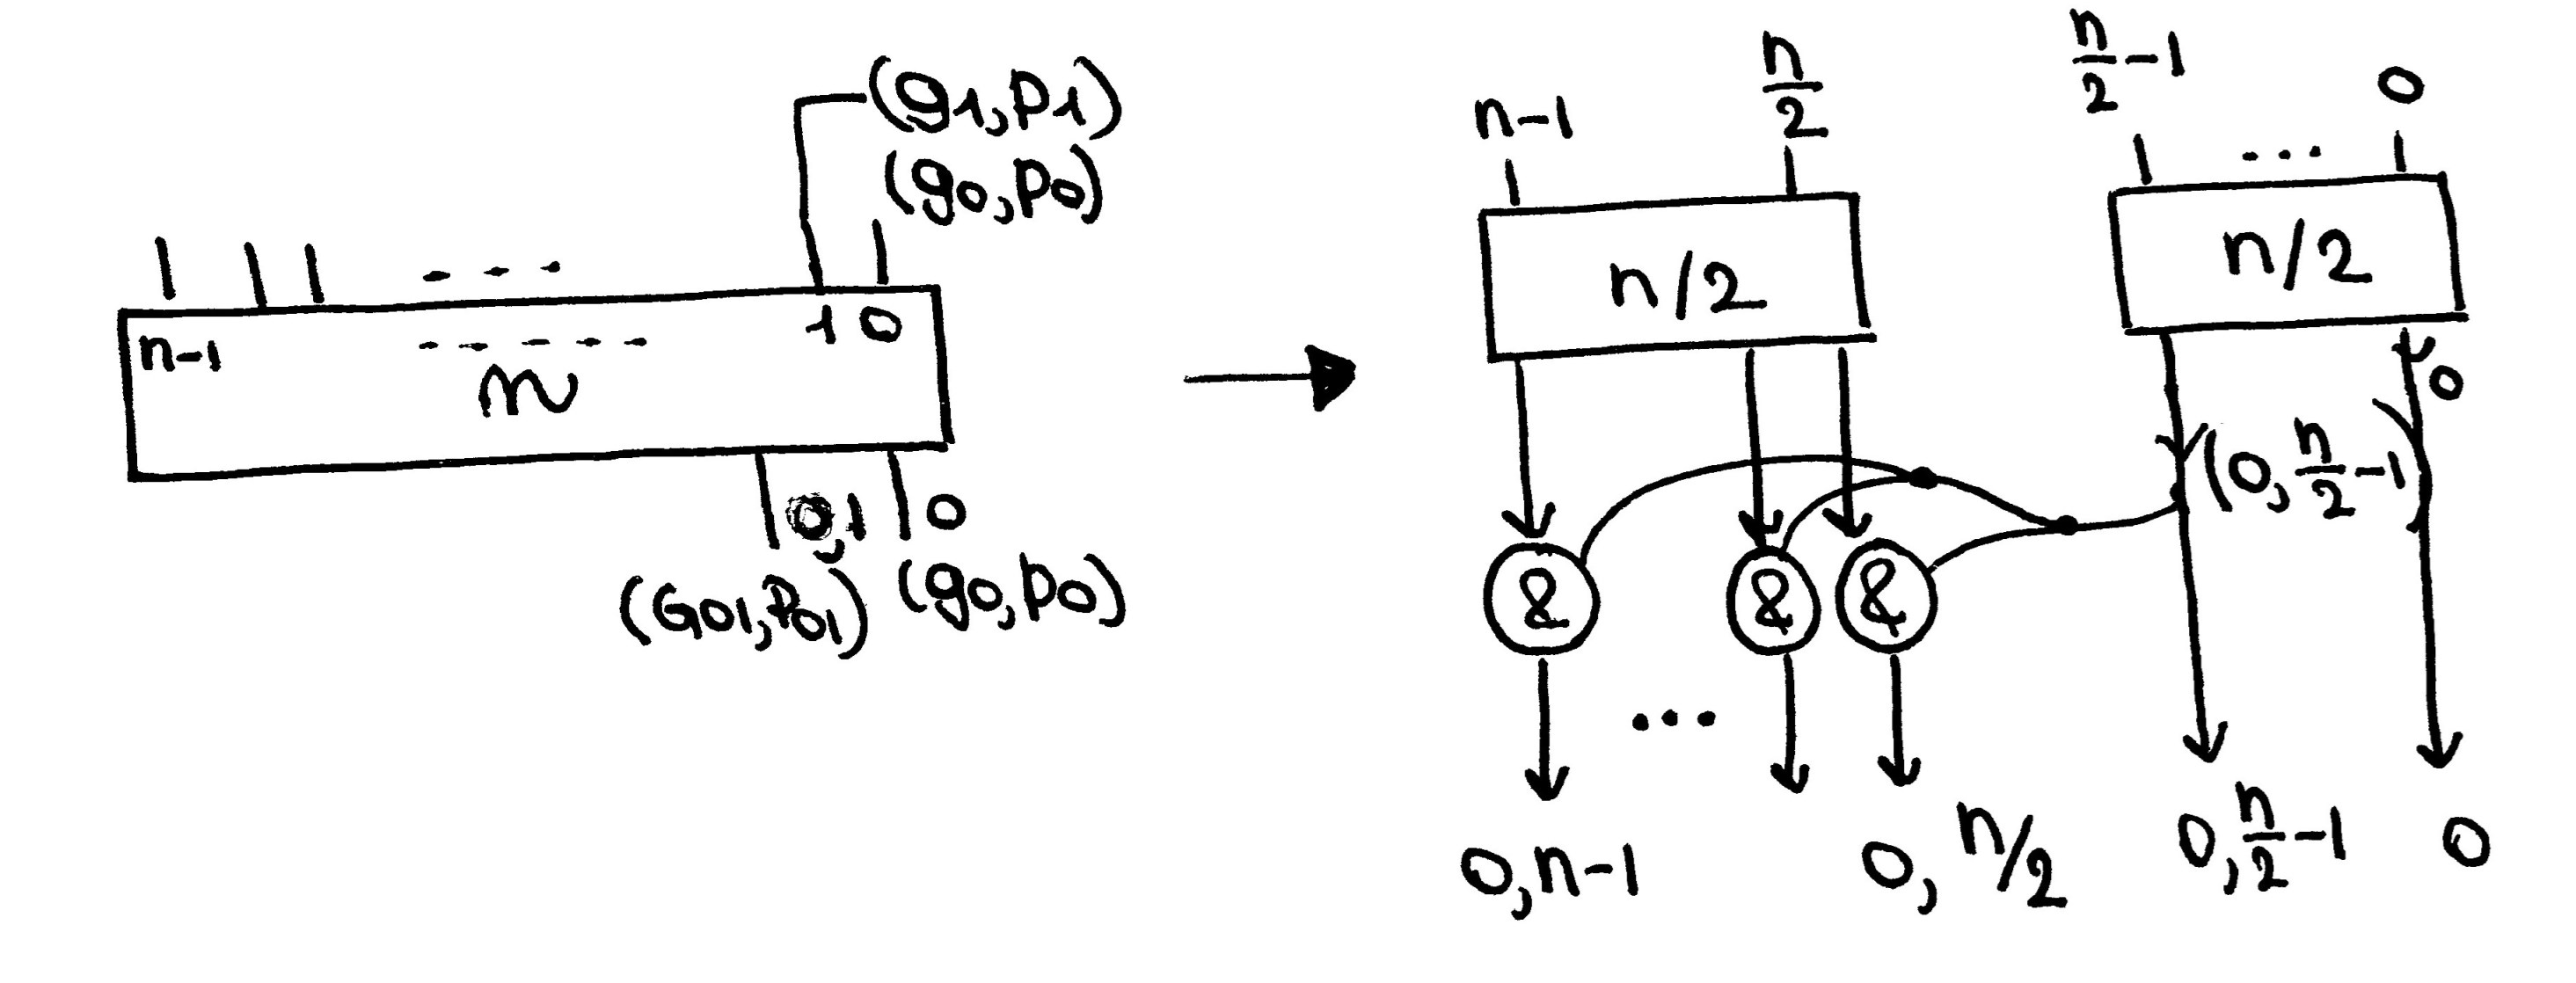
\includegraphics[width=0.7\linewidth]{img/img2/20}
\end{center}
Input set is made up of $n$ samples (for us in position 0 there will be $(g_0, p_0)$) and we expect $n$ outputs where in position 0 there will be just $(g_0, p_0)$, in position 1 (or better (0,1)) we expect $(G_{0,1}, P_{0,1})$ up to last position $(0, n-1)$ corresponding to $(G_{0,n-1}, P_{0,n-1})$.

With this method we split the problem into smaller ones, in the first step we divide the data into 2 blocks, half on one side and half on the other. The first block already gives us a result which is correct, but the second block is proving us data ranging $(n/2, i)$ so starting index is not 0. By combining the first range to the second one using \& operator and replicating this procedure for all subsequent positions, we need to allocate n/2 \& and merge the output of second block with last output of first block.
This is a first solution, then we can allocate for the first block another two blocks each one of n/4 elements and obviously other \& operators.\\

Applying this techniques to $n=8$:

\begin{center}
  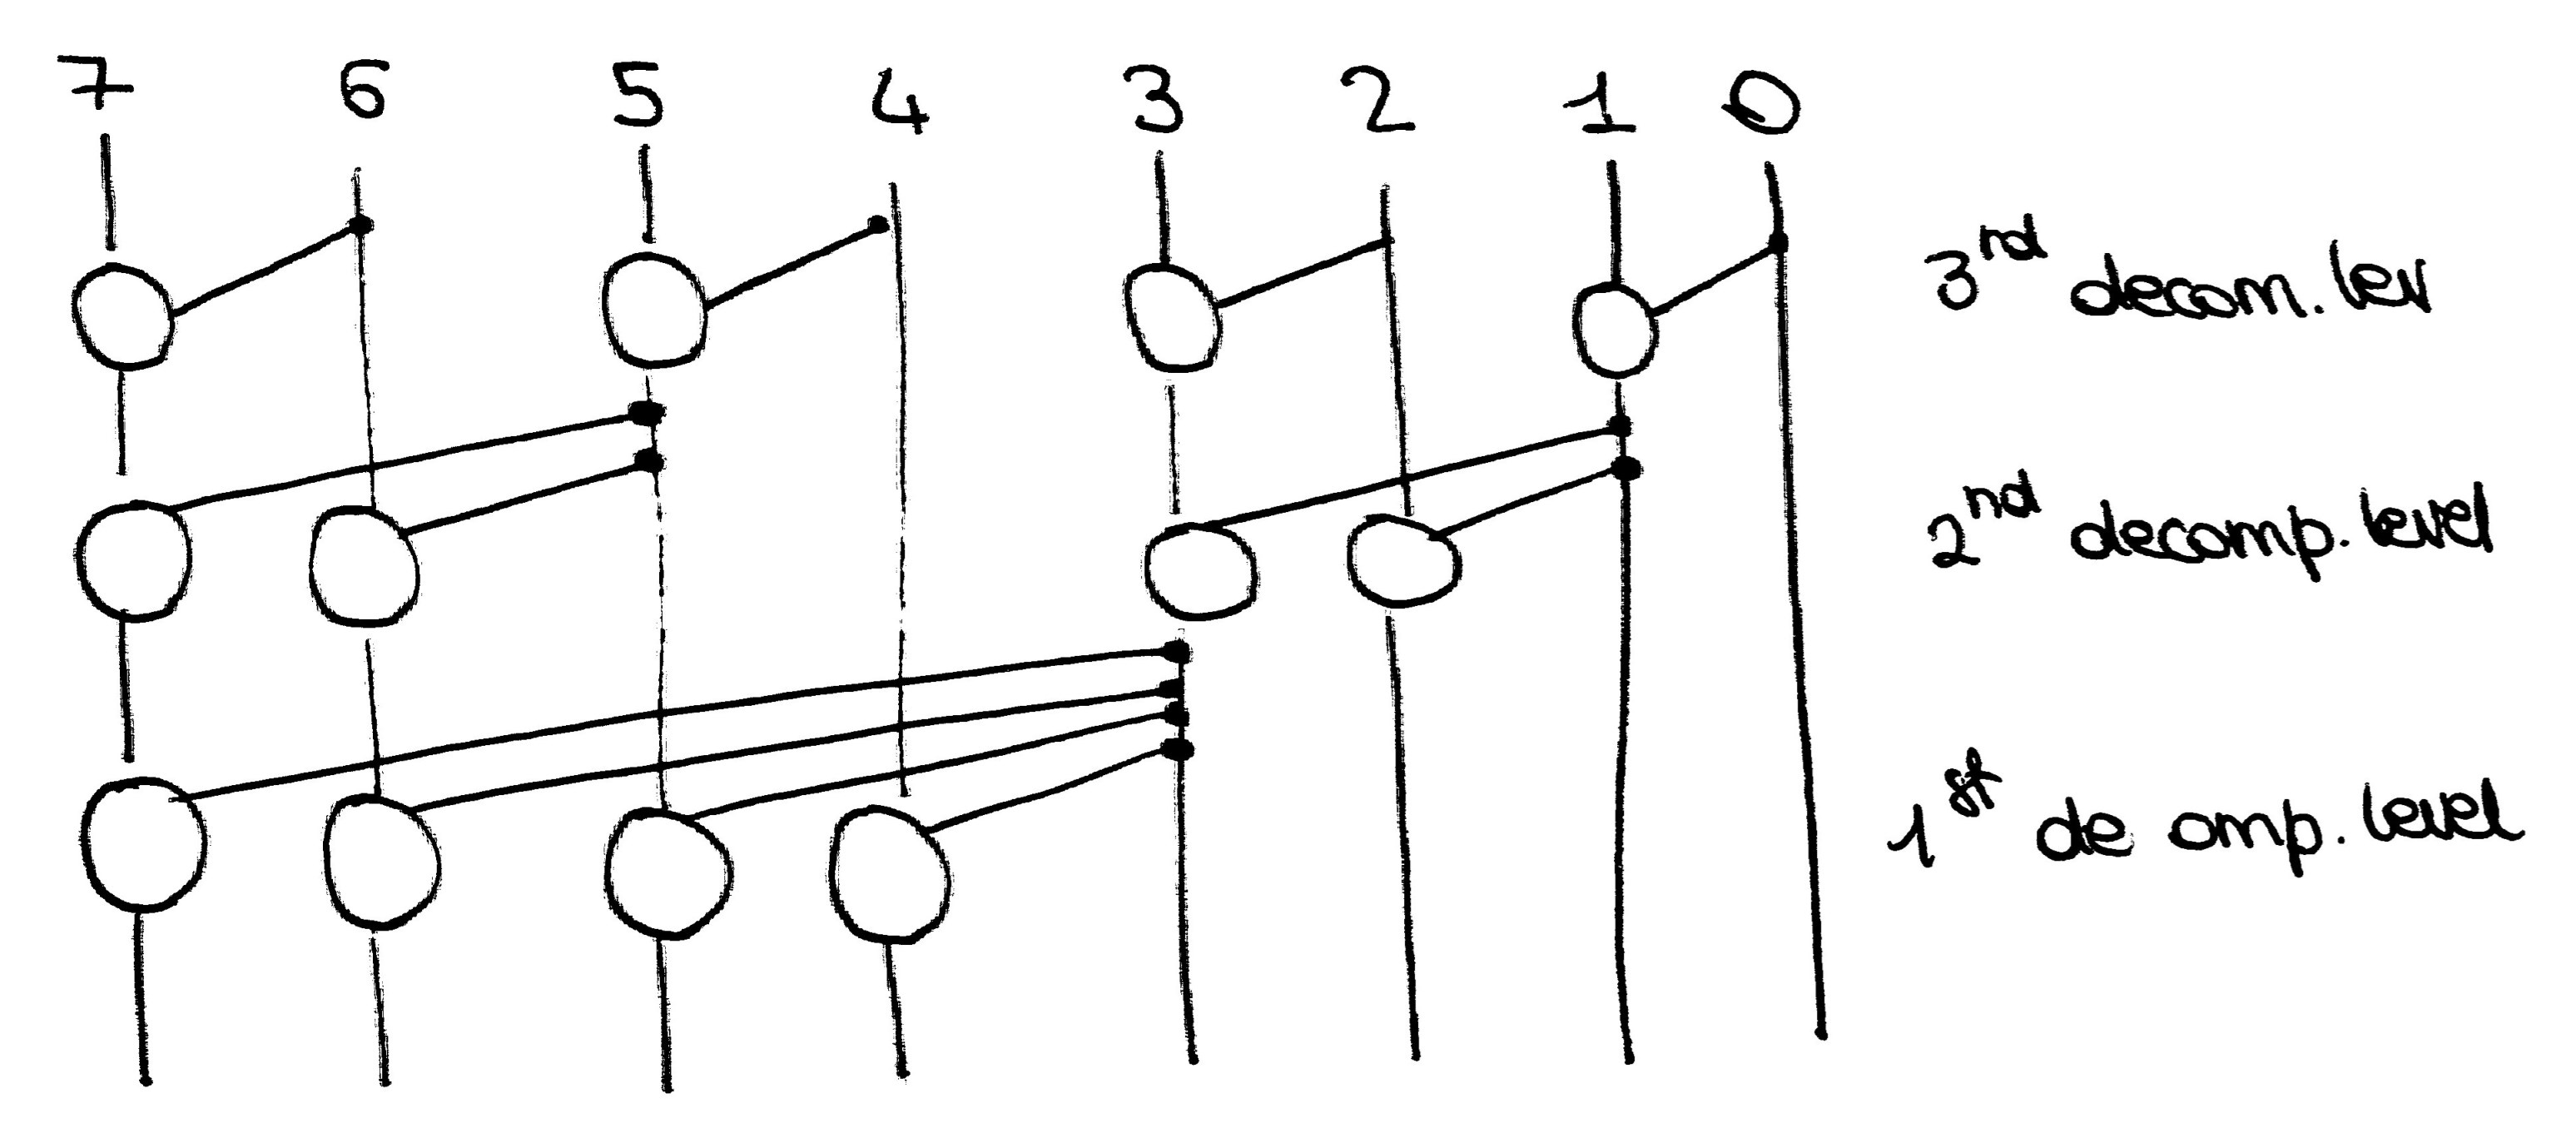
\includegraphics[width=0.7\linewidth]{img/img2/21}
\end{center}

In first level we put all \& between two consecutive inputs making up the third level of decomposition, in second level we start to merge two by two (second level of decomposition)
and in third level the first part is fine while the second part has to be merged with the last outputs of second block, realizing in this way the first level of decomposition.

\subparagraph{Performances evaluation}
\textit{Warning: this is not the complete adder, it only generates G,P starting from g,p but it is actually the most complex part}.\\

\begin{itemize}
  \item \textbf{Complexity} : $ C(n) = $ \#level $\cdot$ \# processing Elements For Each Block $=log_2 (n) \cdot \frac{n}{2}$, so complexity increases linearly with n.
  \item \textbf{Delay} : $ t(n) = $ \# process element we have to go through the critical path = \# levels $= t_{pe} \cdot log_2(n)  $, fine it increases logarithmically.
  \item \textbf{Fan out} : $ F(n) = $ \# process elements that have to be driven from a single point = $= \frac{n}{2}   $, fine it increases logarithmically.

\end{itemize}

Although delay seems to be very low, if $n$ increases in real implementation speed tends to be rather low due to fanout. It seems to be a good solution but with some problems regarding fanout.

\subsection{Brent - Kung}
As before a decomposition of the big problem is performed:

\begin{center}
  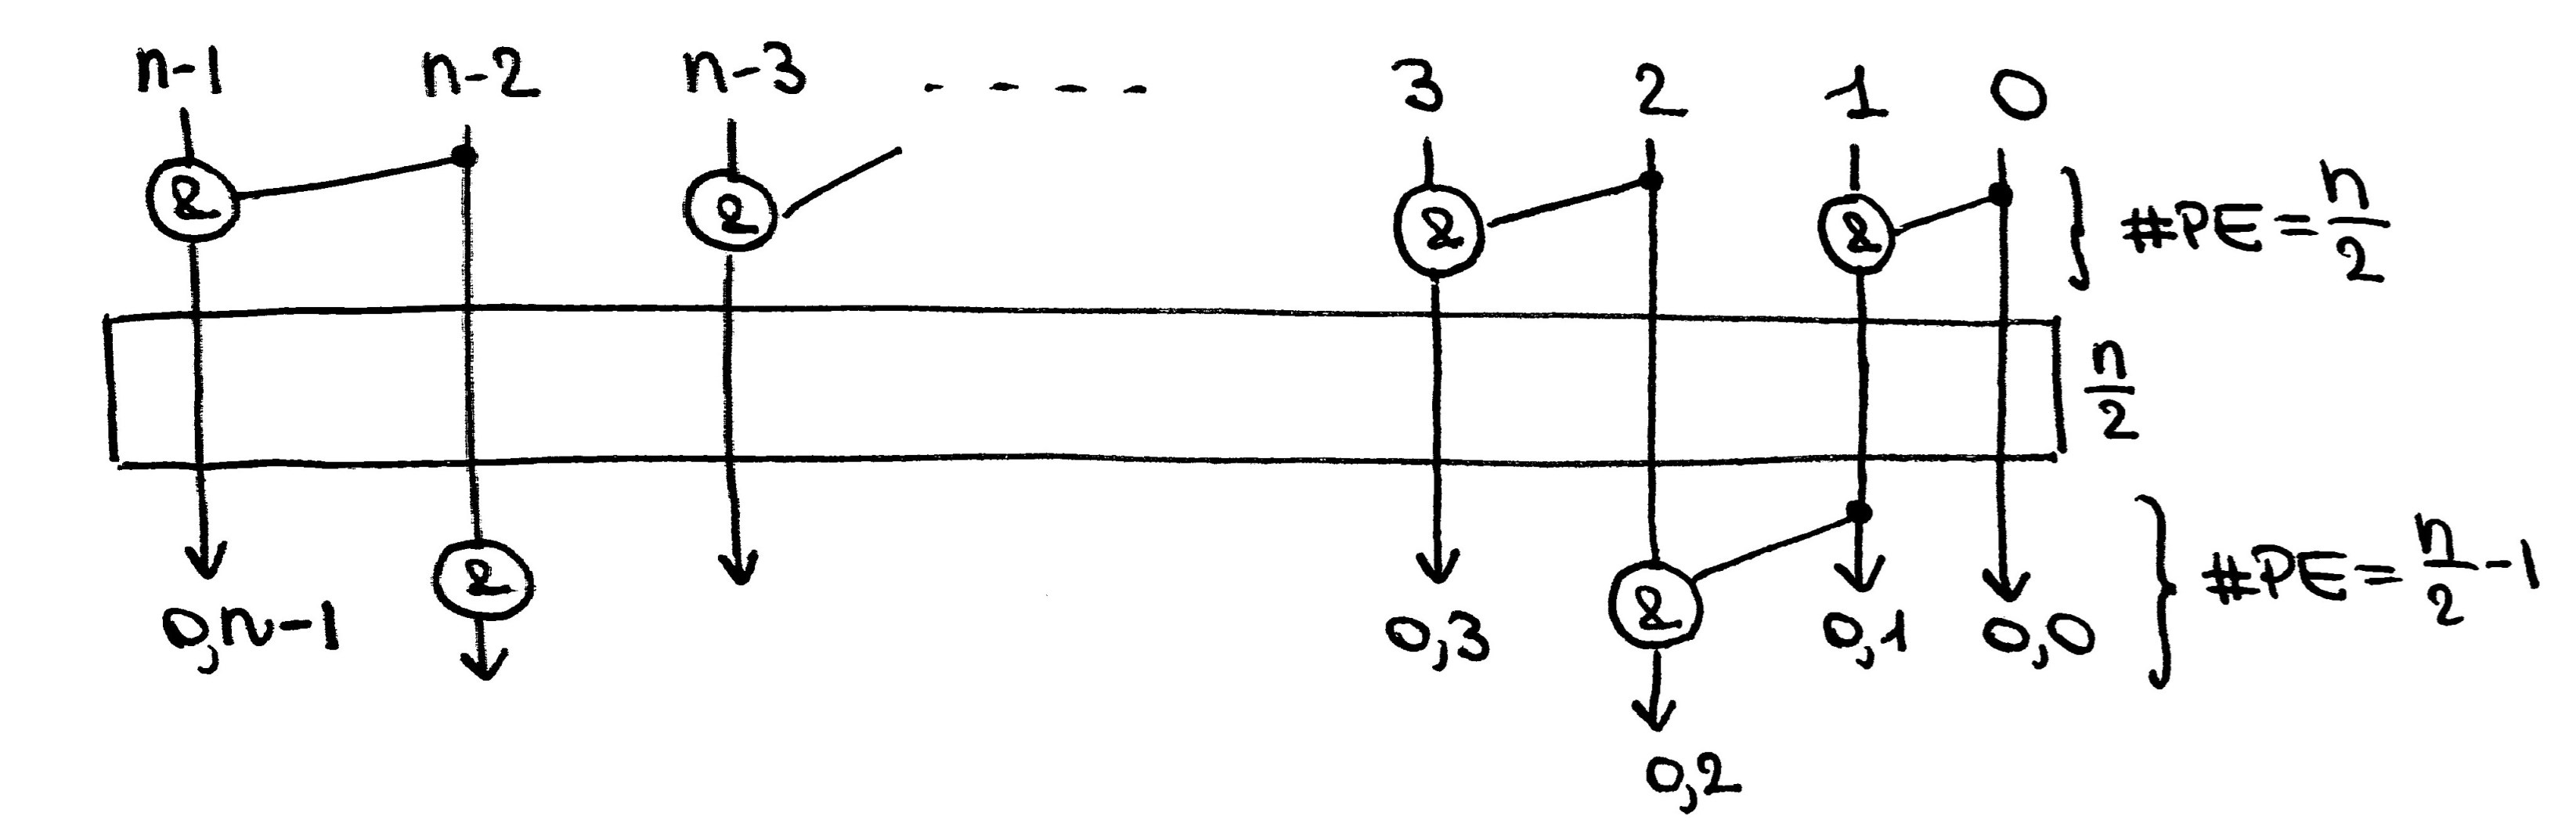
\includegraphics[width=0.7\linewidth]{img/img2/22}
\end{center}

Let's propagate all element in even position while the ones in odd position are processed by a block receiving n/2 inputs (instead of take the first n/2 data, we take one data yes and one not). At the output of inner block we expect (0,1) but we actually have only the first input, so before the input we have to allocate a processing element to merge 0 and 1. For the data in position 2 we need to insert a processing element after the inner block to merge with the output of previous block. This architecture can be completed adding process elements before or after the inner block (before for odd position, after for even position except position 0).\\

The number of processing element we have to allocate for each level of decomposition is $(\frac{n}{2}) + ( \frac{n}{2} -1)$ (before and after inner block). Referring to a complete example:

\begin{center}
  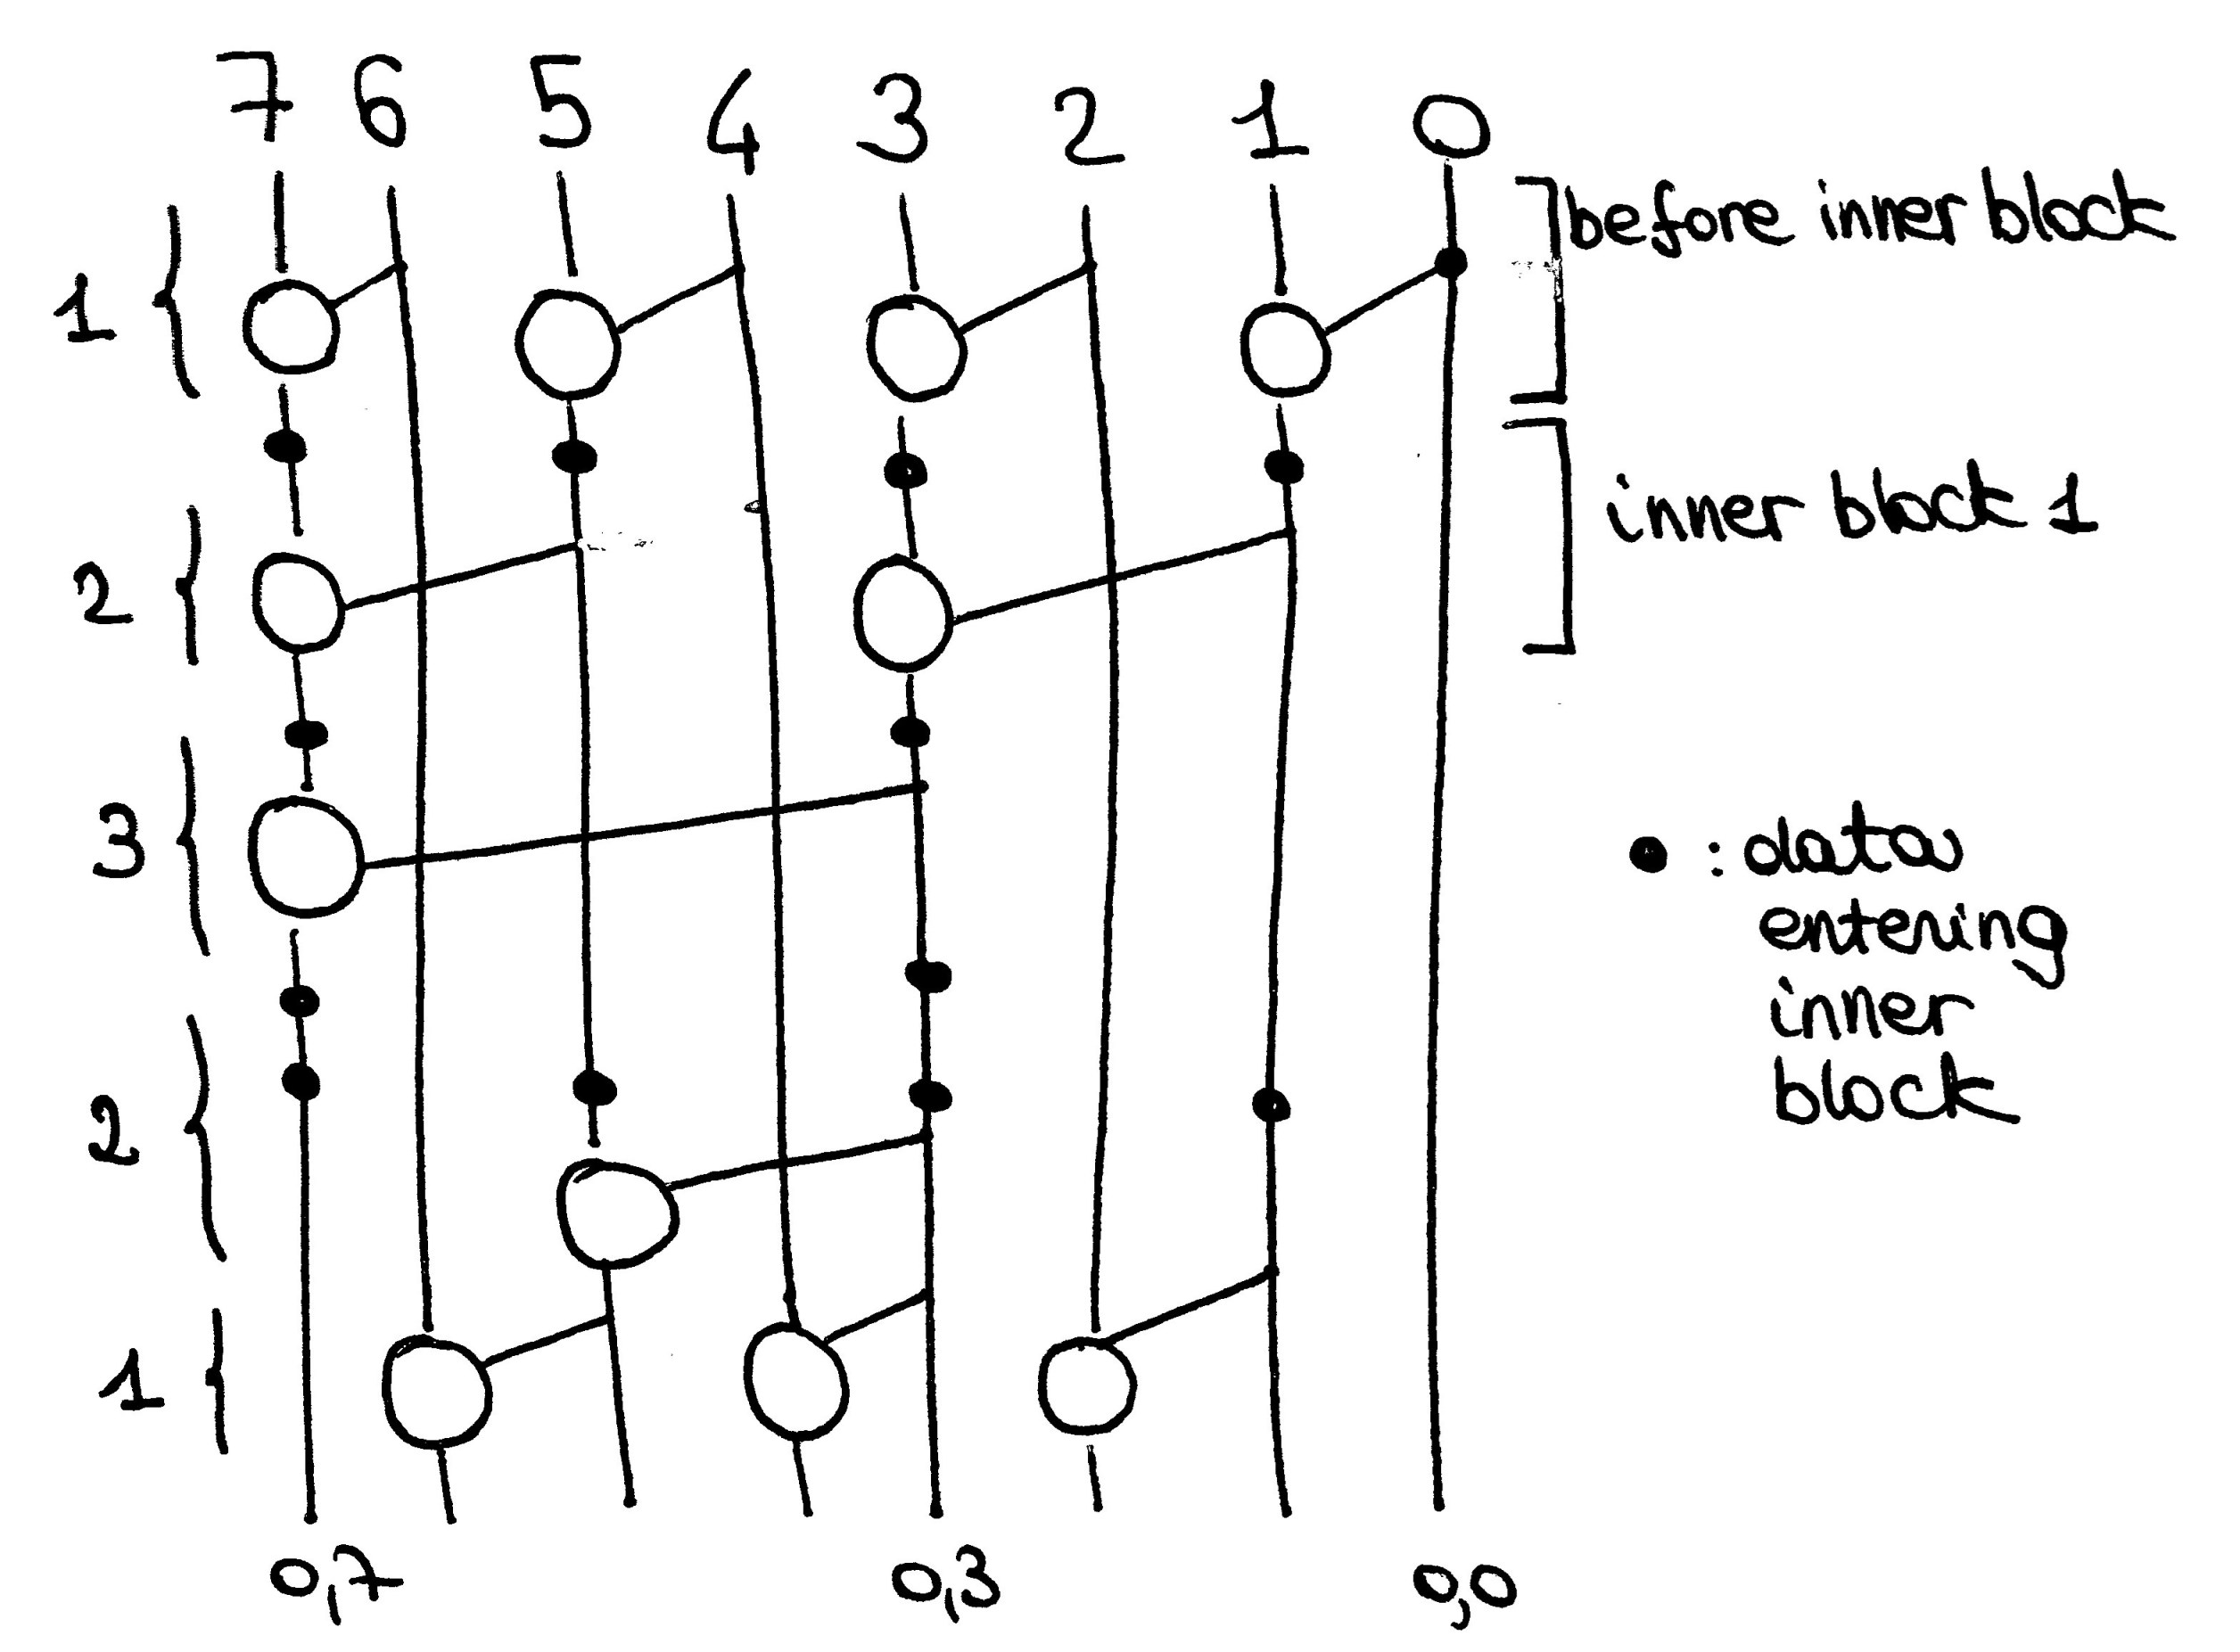
\includegraphics[width=0.7\linewidth]{img/img2/23}
\end{center}

For the second decomposition level no block has to be added at the output, for the first decomposition level we have to place process elements at outputs in even position expect for position zero. Looking at output in position 0 it is already fine, in position 1 we have to combine 0 and 1, in position 2 is fine and so on.

\subparagraph{Performances evaluation}
Regarding complexity, it is:
\begin{eqnarray}
C(n)=C(n/2)+ \#PEs included= C(n/2)+ (n-1)\\
C(n/2)=C(n/4)+(n/2 - 1)\\
..\\
c(n/2^i)=C(n/2^{i-1})+ \frac{n}{2^i}-1\\
\end{eqnarray}

If $k$ is the number of decomposition level, i.e. $k=log_2 n$ then:

$$C(n)=\sum_{i=1}^{k}(\frac{n}{2^i}-1)= n \sum_{i=1}^{k} 2^{-i}-k= 2n-log_2( n) - 2$$

So for $n=8$ $C(n)=11$ (which is one obtained), with respect to Fischer method it's better since it's working as $2n$ and not $nlog_2 n$. For time delay:

$$t(n)=(t_(\frac{n}{2}) + 1 + 1) \cdot (\#innerBlocks -1) = 2log_2 (n) -2$$

Last inner block is not inside the critical path since cp is in the middle. With respect to the previous one, it goes as $2 log$ so it seems worst but looking at fan out:

$$F(n)=log_2 (n)$$

here the fanout is no more increasing linearly.

\subsection{Summarizing}
There are also other networks to solve this problem, summing up together:

\begin{center}
  \begin{tabular}{|l|c|c|c|}
    \hline
    Network&      C(n)&     t(n)&     F(n)\\
    \hline
    Lodner-Fischer&   $0.5nlog_2n$&   $log_2n$&   $n/2$\\
    Brent-Kogge &   $2n-2-log_2n$&    $2log$&     $log_2 n$\\
    Kogge Stone &   $nlog_2n - n+1$&   $log_2$&     $log_2 n$\\
    \hline
  \end{tabular}
\end{center}


In terms of delay only 1 and 3 are the best one, but considering also fanout just last one is better. Looking at complexity the best one is the first one. Depending on technology, we can choose the best one.

\section{Multi-operand adders}

In this situation we are required to sum together partial products or consecutive samples like in a filter, therefore in multipliers and filter multi-operand adders are used. In general we want to sum together $k$ operands each one represented on $n$ bits.

\subparagraph{I idea: sequentially process}
\begin{center}
  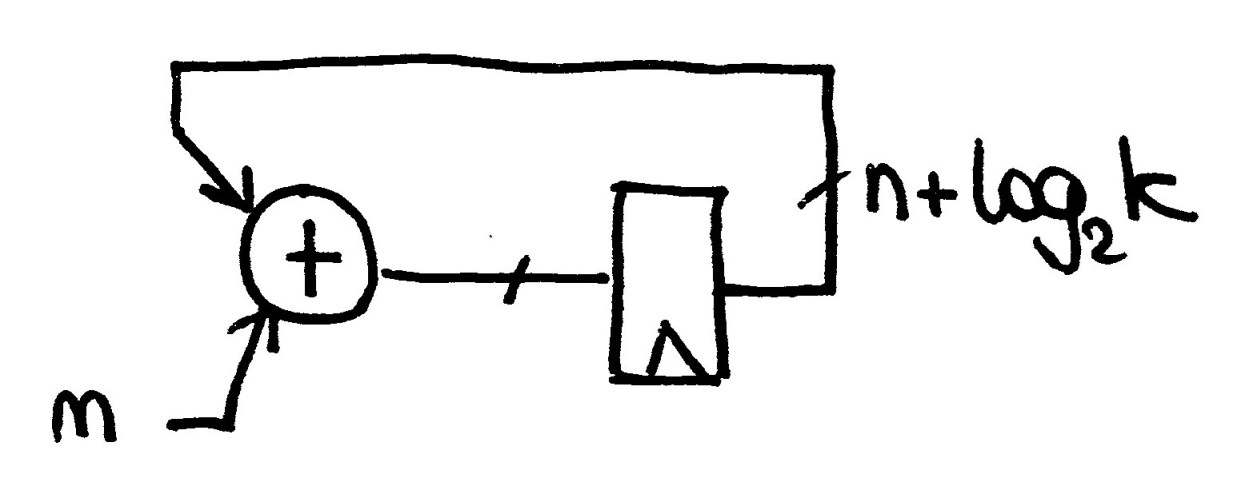
\includegraphics[width=0.5\linewidth]{img/img2/24}
\end{center}

Register and adder have to be sized for the worst case, which is $n+log_2(k)$. An estimation of the total time required is $k(n+log_2(k))$ assuming for adder a RCA.

\subparagraph{II idea: tree-like form  (or in parallel)}
\begin{center}
  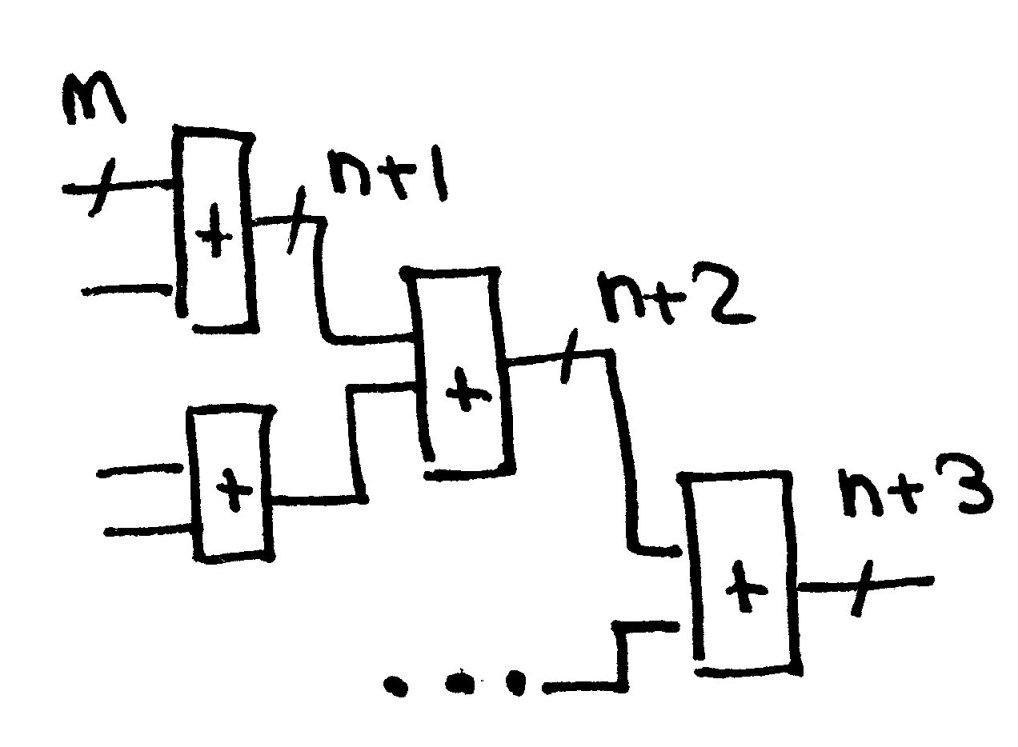
\includegraphics[width=0.5\linewidth]{img/img2/25}
\end{center}

To evaluate critical path we don't have to compute delay adder 1 + delay adder 2+... etc because the adder at second level can start its work when the two least sign bit of the first level are available, meaning that:
$t_{start,1}=0$\\
$t_{start,2}=1$ (1 full adder delay)\\
$t_{start,3}=2$\\
$...$\\

So with $log_2( k)$ levels the last one has to wait for all the previous adder, so along the critical path there are $2log_2 (k)+n$ full adders. This approach is better than sequential one.

\section{Carry save adder (CSA)}

The key idea is to use a full adder as compressor. Let's take a full adder, all inputs are at the same level meaning that they all have the same weight ($a_i,b_i, c_i$) instead for outputs $s_i$ has a weight equal to $2^i$ while carry out has a weight equal to $2^{i+1}$ so it has to be aligned to next full adder.

\begin{center}
  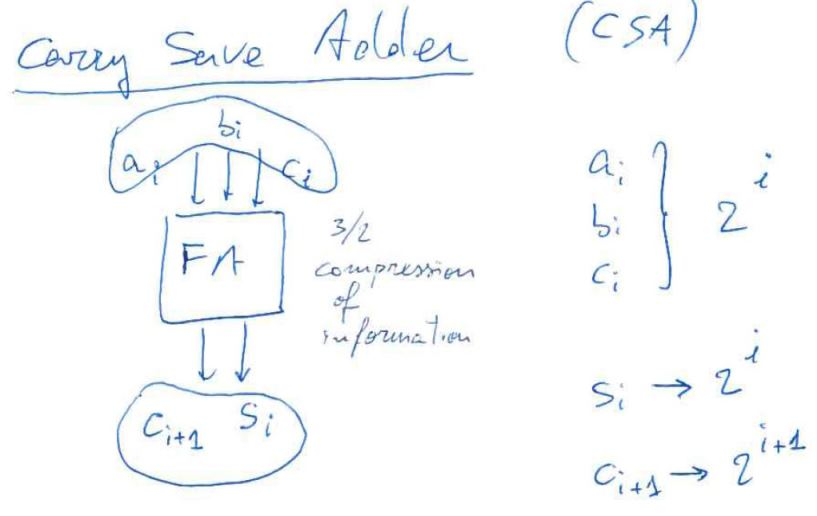
\includegraphics[width=0.7\linewidth]{img/img2/26}
\end{center}
\begin{center}
  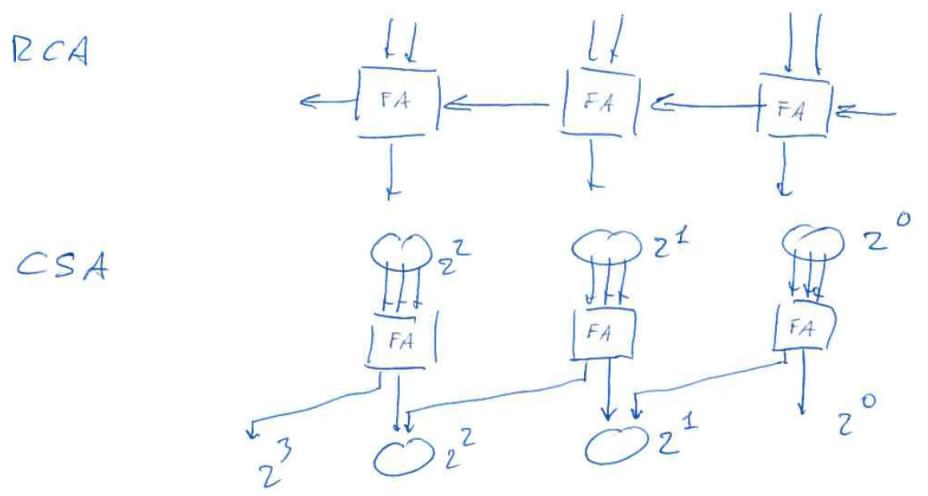
\includegraphics[width=0.7\linewidth]{img/img2/27}
\end{center}

\subparagraph{Example}
\begin{verbatim}
img30














\end{verbatim}
In this case it is $k=7$ so there are 7 operands to be added together (these operands are not on 1 bit only) so we start by adding the first 3 using a CSA (compression of information). Then we take 3 more inputs and the remaining one has to be forwarding with no changes. At the output of CSA we will have 2 stream/CSA. By inserting 4 CSA levels at the end we can obtain only two outputs that can be delivered to a classing 2-input adder.\\

In general if $h$ is the amount of levels needed to deal with $k$ elements, $h(k)$ can be expresses as:
$$h(7)=1+h(\lceil \frac{2}{3}7 \rceil )=1+h(5)$$
where:
\begin{eqnarray}
h(5)=1+h(\lceil \frac{2}{3}5 \rceil )=1+h(4)\\
h(4)=1+h(\lceil \frac{2}{3}4 \rceil )=1+h(3)\\
h(3)=1+h(\lceil \frac{2}{3}3 \rceil )=1+h(2)\\
\end{eqnarray}

since $h(2)=0$ because we don't need anymore a CSA. Every level is introducing a delay equal to the one of a single full adder but we don't have to forget last adder.
Each CSA is a compressor from 3 to 2 so the number of operands decreases as 2/3, integer part.\\

Introducing dot notation we associate the weight of a bit in a certain operand. So in a 7 operand adder, we can describe the operation to be performed as:
$k=7$ is the number of operands while $n=6$ is the parallelism of each operand.
We have to combine bits with same weight, so same weight means same column. Each full adder gives us 1 sum bit which has the same weight as the input plus carry out. For the first level of compression we have sum bit + carry out of the first 2 groups of 3 bit + the last row.
For second level of compression we do the same thing, so if the number of rows is greater than 2 we can continue to compress it.
At third level we see that for the last column we would introduce an additional level of CSA since the carry out of the last CSA would be combined with the other two bits. To avoid it we can use a half adder (the one in dot) to combine two bits which will stay with last carry out. This half adder is not acting as a compressor (2 input, 2 output) but it avoids to have 3 points in the penultimate column. At the end we need:

\begin{center}
  \begin{tabular}{|l|c|c|}
    \hline
    Level&  FAs&  HAs\\
    \hline
    I&    12&   0\\
    II&   6&    0\\
    III&  6&    0\\
    IV&   4&    1\\
    V(RCA)& 5&    2\\
    \hline
  \end{tabular}
\end{center}

Total delay is equal to delay of final RCA plus CSA tree delay (which is equal to number of level multiply the delay of a FA). There are multiple possibilities to distribute FA and HA in the tree, we will do it better when talking on multipliers (Wallace approach: asap allocation of CSA, Dadda approach: a little bit different).

\begin{center}
  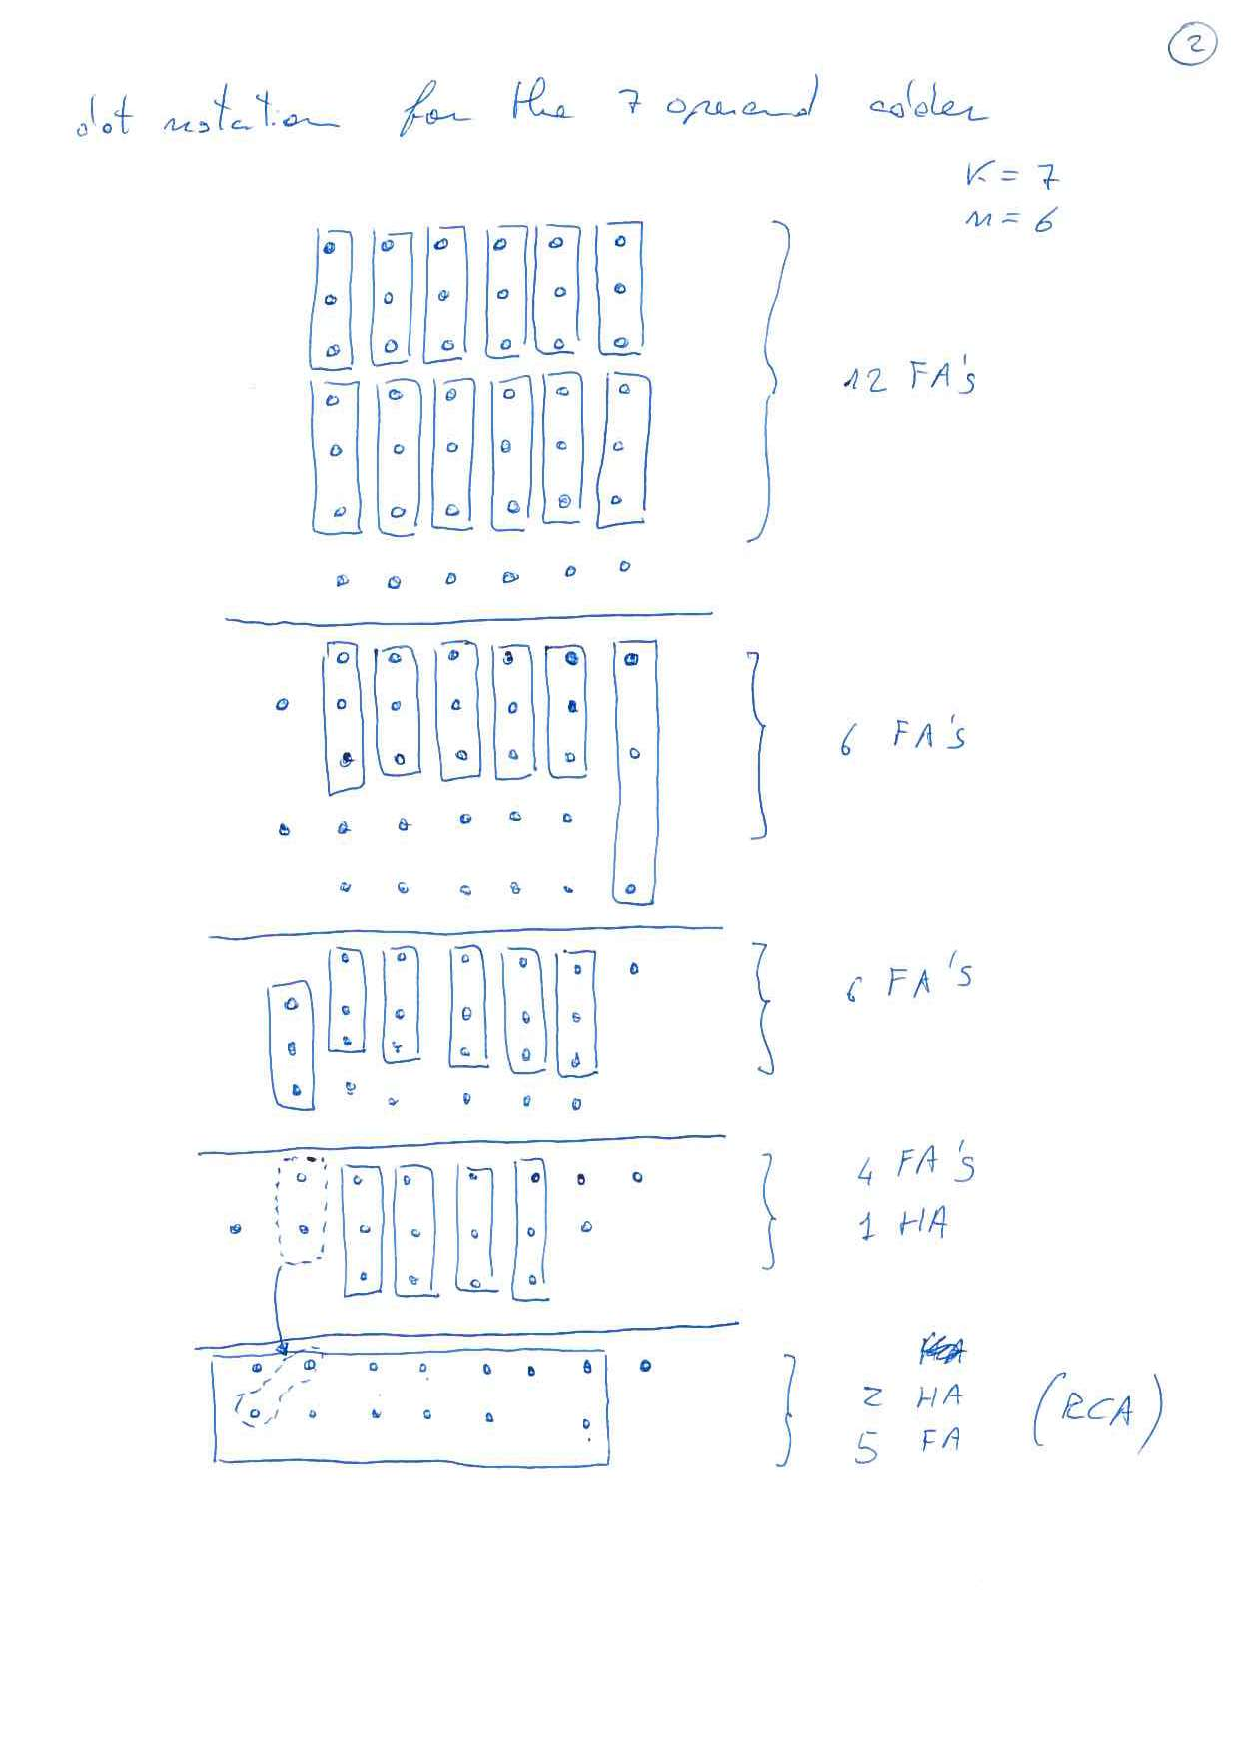
\includegraphics[width=1.0\linewidth]{img/img2/31}
\end{center}


\chapter{Multipliers}

To introduce the adopted notation, it is required to compute $p=a \cdot x$ where:
\begin{itemize}
  \item $a=a_{k-1}...a_0$ is the multiplicand.
  \item $x=x_{k-1}...x_0$ is the multiplier.
  \item $p=p_{2k-1}...p_0$ is the product.

\end{itemize}

As a first approach the pen and paper algorithm will be exploited. Using dot notation:
\begin{verbatim}
img32














\end{verbatim}

In this example $k=4$, after the computation of partial products they need to be shifted and summed together. This implies that a multi-operand sum has to be performed with the difference that with respect to the previous case bits are not aligned but they are always shifted.


\section{Parallel-serial approach}
A first idea to implement this algorithm in HW is to use a parallel/sequence approach: in parallel  all partial products are generated and then they are added serially. Both a top-bottom or bottom-up approach are suitable (right shift or left shift).

\subsection{Right shift approach}
Calling $j$ the number of steps required to accumulate all partial products, it is:

\begin{center}
  \begin{tabular}{|c|c|l|}
    \hline
    j&  Value to be added to acc& Note\\
    \hline
    0&    $a \cdot x_0 \cdot 2^0$&  No shift is required.\\
    1&    $a \cdot x_1 \cdot 2^1$&  It has to be shifted before sum with previous contr.\\
    2&    $a \cdot x_2 \cdot 2^2$&  2 shifts are required to obtain the proper alignment.\\
    ...& ...& ...\\
    \hline
  \end{tabular}
\end{center}

From this approach it comes out that each partial product required a different number of shifts, so a barrel shift should be employed, however since it is a big component with a huge delay we want to avoid it. Let's start from the first partial product and shift all of them by $2^{k-1}$, in this way all contributions have been shifted of the same amount, now when we sum a partial product we shift the value in accumulator of 1 position on the right. In this way we obtain:

\begin{center}
  \begin{tabular}{|c|c|l|}
    \hline
    j&  Value to be added to accumulator& Note\\
    \hline
    0&    $a \cdot x_0 \cdot 2^0$& $a \cdot x_0 \cdot 2^3 =p(0) $ \\
    1&    $a \cdot x_1 \cdot 2^1$& $a \cdot x_1 \cdot 2^3 + (a \cdot x_0 \cdot 2^3) 2^{-1} =p(1) $  \\
    2&    $a \cdot x_2 \cdot 2^2$& $a \cdot x_2 \cdot 2^3 + p(1) 2^{-1} =p(2) $\\
    3&    $a \cdot x_3 \cdot 2^3$& $a \cdot x_3 \cdot 2^3 + p(2) 2^{-1} =p(2) $\\
    \hline
  \end{tabular}
\end{center}

At the end first partial product ($a x_0 2^0$) has been shifted 3 position on the left and 3 position on the right, so it experiences the same amount of shift as in the original algorithm, same thing for the others. With this trick a barrel shifter is no more required.\\

In general we can write that a generic value in the accumulator is equal to:
   $$p(j+1)=p(j)2^{-1}+ax_{j+1} 2^{k-1}$$

From the implementation point of view we will need adder and some shifter.

\subsection{Left shift approach}
Here we start from MSB contribution:

\begin{center}
  \begin{tabular}{|c|c|l|}
    \hline
    j&  Value to be added to accumulator& Note\\
    \hline
    0&    $a \cdot x_3$& \\
    1&    $a \cdot x_2$& $a \cdot x_3 \cdot 2 + a x_2$  \\
    2&    $a \cdot x_1$& $(a \cdot x_3 \cdot 2 + a x_2) 2 + a x_1$\\
    3&    $a \cdot x_0$& $a x_3 2^3 + a x_2 2^2 + a x_1 2^1+a x_0 2^0$\\
    \hline
  \end{tabular}
\end{center}

In this case we need AND gates, adder and 1 shift left. In general:
$$p(j+1)=p(j)2+ax_{k-j-1}$$

\subsection{Architecture}

\subparagraph{Right shift}

\begin{verbatim}
img33














\end{verbatim}

The product is given by the multiplexer: if $x_j$ is equal to 0 we sum 0, otherwise we take $a$.
The adder output will be on $k+1$ bits which are loaded on p-registers shifting them one position to right. In principle we need a $k$ bit adder (even though the final result will be on $2k$ since we are working only on MSB part). We can improve this architecture since we don't need actual a multiplexer since some gates are enough, moreover we can share $k$ LSB bit of p-reg and $k$ bit x-reg: step by step x-reg shifted one position on the right so at the end it will be empty, instead at the beginning LSB part of p-reg is empty and step step it is populated 1 bit/step towards right. So x-reg and p-reg can share the same register.

\subparagraph{Left shift}
\begin{verbatim}
img34














\end{verbatim}

In principle it is quite similar to the previous one, the difference is that x-reg is a left shift reg and we take the MSB bit as multiplexer selector. Partial products are aligned to the right part of p-reg and we need to sum all bits of p-reg, so this time the adder is a 2k adder having double complexity and delay.\\

For left and right shift approaches the same number of steps is required but in the left one the adder will be slower. Moreover in left approach no sharing between x-reg and p-reg is possible. Two algorithms which are very similar lead to quite different hardware implementation.

\subsection{Unsigned division}
If the product is sequence of sum, division is a sequence of subtractions: in principle the architecture is quite close to the one for the product, provided that the adder can perform subtractions.\\

Taking as a example A=111, B=011 we are required to compute Q and R. Using pen and paper approach:

\begin{verbatim}
div













\end{verbatim}

Obtaining Q=010 and R=0001. In hardware it means that:
\begin{verbatim}
img35










\end{verbatim}
B has to be shifted by 2, by 1 and by 0, since we would need a barrel shift B is never shifted but instead we shift A toward left so the relative alignment between A and B is the correct one. Then if the subtraction is positive the corresponding bit of the quotient has to be set to 1 and the result of subtraction is correct, otherwise the bit in Q has to be put to 0 and the result of subtraction has to be discharged.

Summarizing, for each step k:

\begin{itemize}
  \item Substep 1: shift P and A one bit left.
  \item Substep 2: subtract content of B from P and write result on P.
  \item Substep 3: if result < 0, set LSB of A to 0 and restore previous value of P.
  If result >= 0, set LSB of A to 1.
\end{itemize}

At the end what remains in P is the reminder and in A is the quotient.

\section{Signed multiplication}
Again we want to compute $P=AX$ but one of two input operands may be negative.

\subsection{A<0, X>0}
Recalling:
$$P_{j+1}=(P_j+A X_j 2^k)2^{-1}$$
Perform this left shift means take the MSB (the one containing the sign) and report it as new MSB. This is the only change that has to be performed (update sign extension).

\subparagraph{Example}
Let's assume that $A=10110=(-10)_{10}$ and $X=01011=(11)_{10}$. Then:

\begin{verbatim}
ex























\end{verbatim}

Since the result of the sum is not P(i)1 but 2P(i) we have to perform a right shift and the sign bit extension.

While proceeding in the algorithm the word becomes longer and longer. Since A is negative, all partial products are negative. Our final result consists of 10 bit and converted into decimal it should be equal to -110.

\subsection{A positive, X negative}
Since $X<0$ and it is represented in CA2, we can rewrite it as:
$$X=-X_{k-1}2^{k-1}+\sum_{i=0}^{k-2}x_i2^i$$

meaning that for $0...k-2$ we can perform an addition and update the P register as before but for the last contribution (the one associated to $2^{k-1}$) it has the same weight as the position but since it is negative we have to perform a subtraction. The overall architecture doesn't change a lot provided that the adder is also able to perform subtractions. In the last algorithm step we need to complement the output of multiplexer.

\begin{verbatim}
img36














\end{verbatim}

A drawback of this kind of architecture is that it is iterative. When we have a serial topology and we want to go faster we have to exploit a parallel implementation.

\section{Parallel multipliers}

\subsection{Ripple-carry version}
Many solutions exist, we can perform all the partial sum in only one clock cycle by instantiating many adders and making them work in parallel. If we have to compute P=AX and assuming k=4:
\begin{verbatim}
img37














\end{verbatim}

Each column represents a contribution with a certain weight, meaning that $x_0a_0$ is the only one having the lowest weight, $a_1x_0$ has the same weight of $a_0x_1$ and so on. Weight is equal to the sum of indexes, so we have to place partial products in the correct column. Then we can perform a first level of additions: $a_0x_0$ is alone, for $a_0x_1+a_1x_0$ a half adder is enough, for the others full adders are required. By doing it we obtain that this first level is just a RCA.

\subparagraph{Complexity}
Every row is and adder and $k-1$ level of adders are required. By generalizing this structure we have that $k-1$ RCA are required, $k-2$ rows start with HA and end with FA (\# FA=k-1, \# HA =1) while 1 row starts with HA and end with HA (\# FA=k-2, \# HA =2). Therefore complexity:
$$  \#FA_{tot} = (k-2)(k-1)+k-2$$
$$  \#HA_{tot} = k-2+2$$
Complexity increases quadratically with respect to $k$.

\subparagraph{Critical path}
We can follow the last row of full adder from left to right until reach HA of first level of adder. At every change of row we have to add a delay contribution equal to $T_{sum}$, while when changing column we have to add a delay contribution equal to $T_{carry}$. So we have an amount of row changes equals to the number of rows and an amount of column changes equal to last row length. Total delay is therefore:
$$delay=(k-1)t_{sum}+(k-1+k-2)t_{carry}$$
$$delay=(k-1)t_{sum}+(2k-3)t_{carry}$$

Moreover we assume $t_{sum, HA} \simeq T_{sum, FA}$ and $t_{carry, HA} \simeq T_{carry, FA}$ .

How can we be sure that this is the critical path? If now we start from LSB HA of first row and go down until MSB HA of last rows, we have the same number of row and column changes, meaning that actually there are many critical paths with the same length.

\subsection{Carry save version}
Instead of using RCA we exploit carry save adder for each row:
\begin{verbatim}
img38














\end{verbatim}

It is quite close to previous case although here the carry out is not propagated in the same row but is propagated down to the following stage. As in carry save we compress input data up to two operands and then we sum them together using for instance a RCA, or in general a classic adder.

Also here we can find complexity and critical path delay, a key difference with respect to ripple-carry adder version is that here we have one only critical path (because all the others are shorter).

\subsection{Signed operands in parallel approach - Bough Wooley}
A good approach is to use an array of multipliers called Baugh-Wooley.
starting from the definition of product, assuming that A and B are two operands represented in CA2:

$$A=-a_{n-1}2^{n-1}+\sum_{i=0}^{n-2}a_i2^i$$
$$B=-b_{n-1}2^{n-1}+\sum_{i=0}^{n-2}b_i2^i$$

the product will be:

$$P=AB=+a_{n-1}b_{n-1}2^{2n-2}+ \sum_{i}^{n-2} \sum_{j}^{n-2}a_ib_j2^{i+j}-2^{n-1} \sum_{j=0}^{n-2}a_{n-1}b_j2^j - 2^{n-1} \sum_{i=0}^{n-2}b_{n-1}a_i2^i$$

by calling:

$$-2^{n-1} \sum_{j=0}^{n-2}a_{n-1}b_j2^j \rightarrow X  \qquad x_j=a_{n-1}b_j$$
$$- 2^{n-1} \sum_{i=0}^{n-2}b_{n-1}a_i2^i \rightarrow Y \qquad y_i=b_{n-1}a_i$$

Sign will be in position $2n-1$ (MSB for the product), in position $2n-2$ there will be a contribution coming from $a_{n-1}b_{n-1}2^{2n-2}$. For the double sum, if $i=j=0$ then the associated weight is the one related to column 0, then there are all the others contributions and at the end the maximum index is $(n-2+n-2)=2n-4$.

\begin{verbatim}
eq










\end{verbatim}

Ideally we have all bits already in the correct column, provided that X and Y have a minus in front. Instead of perform a subtraction we take their CA2 and perform an addition.

\begin{verbatim}
eq


















\end{verbatim}
The best way is to write all partial products, combine them properly, sometimes contributions have to be taken as they are, other times they have to be complemented. Finally we need to add +1 in column $n$ and $2n-1$. The overall result is an array organization where 2 kind of cell are required:
\begin{enumerate}
  \item AND + FA.
  \item NAND+ FA: before feeding full adder we have to invert the product result (for X and Y).
\end{enumerate}

The point now is how to allocate these cells.

\begin{verbatim}
example 4 bit














\end{verbatim}

A certain bit of coefficient $a$ is linked to all cells in the same column, so now the weight is no more constant inside a column but along diagonals. So sum bit has same weight of related inputs and it is placed along diagonal, carry out bit instead is propagated along vertical direction.
Using this approach the shape becomes square and regular, otherwise each row should be shifted. White cell means no inversion for the product, gray cell implies NAND on inputs.\\

Finally final adder has to be placed so all sums can be performed, moreover we have to consider the addition +1 in positions $2n-1$ and $n$ for CA2. In fact in last RCA two inputs forced at 1 have been added, actually we could force the first one in a HA in the same diagonal, in this way we substitute a FA having carry in equal to one. The second +1 is in the MSB of the product so it is related to the left most diagonal, which is just the last FA of ripple carry adder. In this way we obtain a regular and modular structure, very suitable for VLSI implementation.

\section{Tree multipliers}
The key idea is the use of a CSA which starting from 3 partial products is able to compress the information providing 2 outputs. Therefore by replicating this structure up to the point for which there are no more partial products a tree is build up and a final adder can be employed to compute the product.
\begin{verbatim}
img40






\end{verbatim}

In general three components are employed, i.e.:
\begin{itemize}
  \item PPM : partial products multiplications.
  \item Tree: made up of CSA.
  \item Final 2-input adder.
\end{itemize}

Many approaches exist to obtain a good multiplier, we will see two of them:
\begin{itemize}
  \item Wallace tree multiplier
  \item Dadda tree multiplier.
\end{itemize}

\subsection{Wallace tree multiplier}
It is based on a very simple idea, first all partial products are computed and then:
\begin{enumerate}
  \item Group three rows of partial products.
  \item Move to the following level of the tree those partial products (dots) which don't belong to any group of step 1.
  \item allocate HAs/FAs in order to add together dots in the identified groups.
\end{enumerate}

\subparagraph{Example}
Assuming $n=5$ and having the list of partial products represented in dots notations:
\begin{verbatim}
img41
















\end{verbatim}

At first level we take the first three rows and some up together bit with the same weight (same column) using FAs and 2 HAs. Then we reply these steps up to the point for which only two rows remain.

\begin{center}
  \begin{tabular}{|l|c|c|}
    \hline
     & FA & HA\\
     \hline
     Level 1&   3&    2\\
     Level 2&   4&    2\\
     Level 3&   3&    3\\
     Final RCA&   4&    2\\
     \hline
     Total&     14&   9\\
     \hline
  \end{tabular}
\end{center}

The number of level in the tree is equal to 3.

\subsection{Dadda tree multiplier}
It is very similar to Wallace tree but it tries to allocate HA/FA as late as possible, in fact we can postpone in time the allocation of a component provided that the number of levels does not increase. Instead in Wallace tree the allocation of resources was made as soon as possible.\\

Firstly some values have to be evaluated, in particular $d_j$ indicates the number of operands to be handled at level j. So in the last level $d_1$ is equal to 2 since in the end we want to have just two rows to be added together with a classic adder, for previous levels it is

$$d_{j+1} = \lfloor 1.5 d_j \rfloor$$

where 1.5 is the compression factor. So it will be: $d_2=3; d_3=4; d_4=6$.\\

At level j we allocate HA/FA in order to achieve in the following level a number of operands not bigger than $d_{j-1}$ meaning that we want to reduce the amount of operands from $d_j$ to $d_{j-1}$. By doing that we also have to consider carry bits since when we allocate a FA we compress from 3 to 1 bit dots in the same column but we also generate a carry out bit which was not present previously.

\subparagraph{Example (the same as before)}

\begin{verbatim}
img42


























\end{verbatim}

since we start from a number of operands equal to 5 we have to take as initial level $d_4=6$ (the integer just up) and as first step we have to reduce from 5 to 4. Every column which has less than 5 elements has to be ignored since we want at the next level no more than 4 rows. It doesn't matter if we can decreases it more, we have to allocate the minimum HW to reach 4 rows by postponing the compression.\\

In first level we start with column number 4 and putting a HA is enough to compress from 5 to 4. Apparently in column 5 there is no need to allocate anything however due to HA in previous column a carry out bit is generated which go in column \#5 and increases its number of bits, this implies that we have to allocate a HA in order to have 4 bit in column \#5. In second level we have to move from 4 bit/column to 3, so we start with 1 HA and then FA. \\

\textit{Issue}: we are decreasing the number of rows at the same rate as in Wallace tree but with much less hardware.

At the end we have the RCA which is more complex than the one in Wallace, in fact here we spend less resources in tree but more in RCA, while in Wallace we have more resources in the tree and the final adder was easier.

 \begin{center}
  \begin{tabular}{|l|c|c|}
    \hline
    & FA & HA\\
    \hline
    Level 4&    0&    2\\
    Level 3&    3&    1\\
    Level 2&    5&    1\\
    Level 1&    8&    0\\
    \hline
    Total&      15&   5\\
    \hline
  \end{tabular}
 \end{center}

Complexity is a little bit lower for Dadda tree, in fact by increasing bits number the difference between Wallace and Dadda increases and Dadda results in cheaper implementation.
In terms of equivalent gates, the following table takes into account not only the tree but also the final RCA.

\begin{center}
  \begin{tabular}{|l|c|c|c|c|}
    \hline
    & Complexity & & Delay &\\
    & Wallace & Dadda& Wallace& Dadda\\
    \hline
    4x4&    104&    104&    21&     19 \\
    8x8&    552&    528&    42&     37 \\
    16x16&    2476&   2336&   77&     69 \\
    32x32&    10283&    9792&   145&    133 \\
    \hline
  \end{tabular}
\end{center}

Both in term of complexity and delay there is some advantages in using Dadda tree. These kind of multipliers can be pipelined, i.e. applying pipeling to CSA performance increases a lot as well as latency.

\section{Booth multiplier}

Starting from binary numbers they can be simplified by using a different representation. For instance if we have to compute  $15 \cdot A$, using a binary representation the coefficient 15 would be expressed uniquely as "001111". Let's suppose to have an internal extended alphabet made up of ${0,1,\overline{1}}$, now to represent 15 many possibilities exist:

\begin{center}
  \begin{tabular}{|c|c|c|c|c|c|c|c|}
    \hline
     & & & & & & Value & Required operations\\
    \hline
    0&  0&  1&  1&  1&  1&        $P=A+2A+4A+8A$&   3 additions\\
    0&  1&  0&  0&  0&  $\overline{1}$& $P=16A-A$&      1 difference\\
    \hline
  \end{tabular}
\end{center}

The advantages of using this representation allow to reduce a lot complexity in case we want to perform multiplication since it becomes just a series of sums properly shifted. This idea can be exploited to obtain adders based on this algorithm

\subsection{Booth algorithm}
Two consecutive digits are analyzed at the same time, in particular we notice that:
\begin{center}
\begin{tabular}{|c|c|c|c|}
  \hline
  $x_i$&  $x_{i+1}$&  What they represent&  Operation to be performed\\
  \hline
  0&    0&      in middle of sequence&  -\\
  1&    1&      in middle of sequence&  -\\
  1&    0&      Tail of sequence&   $-A \cdot 2^i$\\
  0&    1&      Head of sequence&   $+A \cdot 2^i$\\
  \hline
\end{tabular}
\end{center}
\subparagraph{Example}

Again we start from 15 whose binary representation is "00111". In LSB a dummy zero is inserted to recognize the tail of sequence of ones. We are shifting the window (| |) one position to the left by the time, windows of consecutive steps are overlapping.
\begin{center}
\begin{tabular}{|c|c|c|c|c|c|c|c|c|}
  \hline
  Step (i)& & & & & & & & Operation to be performed\\
  \hline
    0&    0&    0&  1&  1&  1&  |1& 0|&   $-A$\\
    1&    0&    0&  1&  1&  |1&  1|&  0&    nop\\
    2&    0&    0&  1&  |1&   1|&  1& 0&    nop\\
    3&    0&    0&  |1& 1|&   1&   1& 0&    nop\\
    1&    0&    |0& 1|& 1&    1&   1& 0&    $+A \cdot 2^4$\\
  \hline
\end{tabular}
\end{center}
Since in MSB positions we have only zeros no further operations have to be performed. Actually we can apply this algorithm also to numbers like "0010" resulting in $"01\overline{1}0"$. This is an interactive algorithm, so by looking at more than two-bit at the same time to speed up the executions. This approach leads to radix-4 version whose truth table is the following:
\begin{center}
\begin{tabular}{|c|c|c|c|c|}
  \hline
  $x_{i+1}$&    $x_i$&  $x_{i+1}$&  What they represent& Operation\\
  \hline
  0&        0&    0&      -&          -\\
  0&        0&    1&      head& $+A2^i$\\
  0&        1&    0&      head + tail, sequence of length 1&   $+A2^{i+1}-A2^i=A2^i$\\
  0&        1&    1&      head&  $+A2^{i+1}$\\
  1&        0&    0&      tail&  $-A2^{i+1}$\\
  1&        0&    1&      head + tail&  $-A2^i$\\
  1&        1&    0&      tail&  $-A2^i$\\
  1&        1&    1&      -& -\\
  \hline
\end{tabular}
\end{center}
Applying radix 4 to previous example (always inserting dummy bit in LSB):
\begin{center}
\begin{tabular}{|l|c|c|c|c|c|c|c|c|}
  \hline
  Position&   5&  4&  3&  2&  1&  0&   Operation\\
  \hline
  i=0&    0&  0&  1&  1&  |1& 1&  0|&   $-A2^0$\\
  i=2&    0&  0&  |1& 1&  1|& 1&  0&    $nop$\\
  i=4&    |0&  0& 1|& 1&  1&  1&  0&    $+ A 2^4$\\
  \hline
\end{tabular}
\end{center}
Same result as before but with only 3 steps, so in general using radix-4 we divided by two the number of steps required.
The Booth algorithm can be implement sequentially or in parallel.

\subsection{Sequential approach}

\begin{verbatim}
img43














\end{verbatim}

After multiplex we would need a barrel shift to shift to the left $A, -A, 2A, -2A$ by a value depending on the current step. Since we don't want to use that component we postpone the shift to the accumulator in the opposite directions (right shift). Since it is an iterative algorithm using unrolling we should be able to parallelize it (try to think how to achieve that).

\chapter{Dividers}
The aim is to evaluate quotient and reminder starting from two input data, by calling:
\begin{itemize}
  \item $z$: dividend (2k bits).
  \item $d$: divisor  (k bits).
  \item $q$: quotient (k bits).
  \item $r$: reminder  (k bits). % il reminder è r o s???
\end{itemize}

The outputs will be:
$$\frac{z}{d}=q+(\frac{r}{d})$$
$$r=z-dq$$

\section{Pen and paper approach}

Let's assume $k=4$ bit:

\begin{verbatim}
img44











\end{verbatim}

Each partial product experiences a different shift, to avoid the allocation of a barrel shifter we can exploit the same idea of the multiplier, i.e. shift everything by $2^k$ and then shift only by one position at the time the partial reminder, in this way 2 fixed-amount shifters are sufficient.

$$s^{(0)}=z , s^{(j)}=2s^{(j-1)}-q_{k-j}d2^k$$

Relative position of partial reminder is the same as in the pen and paper algorithm, in the last step we have to:
$$s^{(0)}=s2^k$$

\subparagraph{Example}
By considering $k=4$, $z=(117)_{10}=(01110101)_2$ and $d=(10)_{10}=(00001010)_2$:

\begin{verbatim}
ex























\end{verbatim}

The architecture can be simplify as follows:

\begin{verbatim}
img45














\end{verbatim}

The critical point is the data dependency we have in these steps, in particular we cannot save the partial reminder before testing $C_{out}$, so the critical path will not just be the longest one but we also need a control unit that receiving $C_{out}$ it eventually asserts the shifter load signal. This solution (known as restoring version) can be improved.

\subsection{Restoring and non restoring}

Looking at the previous example, we have to perform comparisons like
$2s^{(1)}-d2^4 <0$. Depending on sign value we decide to store or not the difference result as new partial product, however it may become the bottleneck. Two different approaches can be exploited:

\begin{enumerate}
  \item \textbf{Restoring approach}: from an algebraic point of view in order to restore the previous partial product we can perform:
  $$ 2s^{(1)}-d2^4+2^4d=s^{2}=2s^{(1)}$$
  So in next stage:
  $$ 2s^{(2)}-d2^4=4s^{(1)}-2^4 d$$

  \item \textbf{Non-restoring approach}: we don't test immediately $C_{out}$ but we store the result independently if it negative or not. With respect to previous approach, no additional delay due to carry out propagation is introduced however the result is not correct. The idea is try to correct it in the following step:
  $$2s^{(1)}-d2^4=s^{2}$$
\end{enumerate}

\subparagraph{Non-restoring}
We understand that in the following step we don't perform anymore a subtraction but an addition in the case of negative previous reminder, to compensate the current wrong result.

$$2^{(2)}+2^4 d=4s^{(1)}-2 2^4 d + 2^4 d = 4s^{(1)} -2^4d$$

Since we obtain the same result as in the first approach it means that $C_{out}$ test can be delayed of 1 clock cycle, so we have more time to perform this operation and it is no more the bottleneck. In this way the delay is the one of the adder and control-unit is no more needed, therefore this last implementation leads to a much better design.

In case of negative result at the very last step probably some more computations are required to recover the correct reminder. Since it is the last step of the algorithm, we have no more steps to recover it, meaning that we have to perform a final test on the last step, if the reminder is negative we have to perform an extra-step to compensate the error; in the end each iteration will be faster but maybe an extra step has to be considered, usually this trade off is more than acceptable.

\subparagraph{Example 107/10}

\begin{verbatim}
ex























\end{verbatim}

\section{Signed division}

\subsection{BSD representation}
In a generic step $s^{(j)}$ may be $\geq 0$ so  $q_{k-j}=1$ or $<$, in this case instead of putting $q_{k-j}=0$ we decide to assign the value '-1', in this way usual binary digit set is replaced with ${0,1} \rightarrow {-1, 1}$. Starting from now $q$ value will be represented in this new set, called BSD (\textbf{Binary Signed Digit}).\\

The conversion from BSD to binary can be performed using a 4-steps algorithm:
\begin{enumerate}
  \item Replace all digits equal to "-1" with "0".
  \item Shift one bit to the left.
  \item Complement the MSB.
  \item Add 1 in the least significant position.
\end{enumerate}

As an example let's consider $(11)_{10}$ corresponding to:
\begin{verbatim}
    1 1 -1  1   // start, in BSD 13-2=11
    1 1 0 1   // step 1
 1  1 0 1 -   // step 2
 0  1 0 1 -   // step 3
 0  1 0 1 1   // step 4
\end{verbatim}

The final result is expressed as usual and it is equal to 11. This is useful in signed division.

\subsection{Signed division algorithm}

We expect that $sign(s)=sign(z)$ i.e. the sign of the reminder must be equal to the sign of the dividend and that $sign(q)=sign(z) \oplus sign(d)$. Restoring algorithm can be reused leading to the well known recursive expression:
$$s^{(j)}=2s^{(j-1)}-q_{k-j}d2^k$$

If $sign(s^{(j-1)}) \neq sign(d)$ instead of performing a subtraction we have to perform an additions, in this way we can proceed with same steps as in unsigned case. Depending on divisor sign for each step :
\begin{itemize}
  \item If $d>0$:
    \subitem if $s^{(j-1)} \geq 0$ then $q=1$ and a subtraction has be performed.
    \subitem if $s^{(j-1)} < 0$ then $q=-1$ and an addition has be performed.
  \item If $d<0$:
    \subitem if $s^{(j-1)} \geq 0$ then $q=-1$ and an addition has be performed.
    \subitem if $s^{(j-1)} < 0$ then $q=1$ and a subtraction has be performed.
\end{itemize}

If at the end the sign of partial reminder is not correct again we have to perform an extra step to achieve a correct result for it.\\

So far we have considered unsigned/signed shift and subtraction operations for the division using a iterative approach. How can we achieve a faster division?

\section{Fast division}
Two different approaches can be exploited:
\begin{enumerate}
  \item Same as before but as fast as possible: choose fast adders/subtracters but the algorithm remains iterative.
  \item Try to reduce the number of iterations leading to radix-approach.
\end{enumerate}

So far the amount of required iterations was equal to $k$ since we evaluated 1 bit at the time (radix-2), the idea is to compute 2 bits/iteration in order to obtain ideally a double faster execution (radix-4). It is also possible evaluate 3 bits/iteration (radix-8). In general in order to employ a radix approach we have to substitute in last expression '2' with 'r', leading to:

$$s^{j}=rs^{(j-1)}-q_{k-j} (r^k d)$$

\begin{verbatim}
img46














\end{verbatim}

Bn applying this approach the key architecture is more or less quite similar to the original one. The problem is to guess the correct value for $q_j$ since before it was just 0 or 1, now there are 4 possibilities at each iteration and depending on the reminder sign we have to determine the correct one, in principle we should determine 4 partial products, perform the subtraction and then see which of these 4 has a plus sign. A solution may be simplify the guess of digits by employing an extended digit set.

\subparagraph{Example (base 10)}

\begin{verbatim}
img47














\end{verbatim}
In the first step we take the 2 MSB of z and 1 MSB of d, so $12/2=6$ and although MSB of q is wrong we ignore this fact and keep it, then we proceed with the reminder, we obtain a negative reminder so instead of choose a different value for 6 we actually go on and choose as second digit -3, then we perform the same computations obtaining a positive reminder which is actually the correct one. For the reminder we have $= 6 -3$ which is $6 \cdot 10+(-3) \cdot 1=57$. We decide to accept wrong values during computations since we are using a different digit set (the one that also included negative value).

\subparagraph{Array based solution}

\begin{verbatim}
img48



















\end{verbatim}

In first row the difference between $z$ and $d$ shifted of 4 position is performed since carry in of the first adder is 1 and the exor is complementing $d$. In second row:ì depending on $q_3$ sign we perform an addition or a subtraction.
Array based divider is able to perform the whole shift and subtract algorithm, however it's fully combinational with a huge delay, since each row is actually a RCA. Overall total delay is equal to $k^2 \cdot delay_{single,adder}$ so it is in quadratic relationship with respect to $k$. To speed up the execution is possible to pipeline, in particular if we have to perform a lot of divisions one after the other it is a very good solution, especially for throughput (not for latency since it is very high).

\section{Division by repeated multiplications}

One more additional idea to implement division:

$$q=\frac{z}{d}=\frac{z x^{0} x^{1}... x^{m-1}}{d x^{0} x^{1}... x^{m-1}}$$

The key idea is to multiply $z$ and $d$ by different values, a part for the precision this approach can be employed only if at the end we guarantee that $d x^{0} x^{1}... x^{m-1}$ is equal to 1 then $z x^{0} x^{1}... x^{m-1}$ will be equal to $q$.

The points are:
\begin{itemize}
  \item Number of iterations required.
  \item Sequence of $x$ values guaranteeing the result.
\end{itemize}

By defining $d^{(0)}=d$ then $d^{(i+1)}=d^{(i)}x^{(i)}$ and $z^{(i+1)}=z^{(i)}x^{(i)}$.

We obtain a reasonable result by choosing for $x$ the reciprocal of d (to have at the end $x \cdot d \simeq 1$), in this condition we can approximate $1/d=x$ with its tangent:

\begin{eqnarray}
x^{(i)}=2-d^{(i)}\\
d^{(i+1)}=d^{(i)} x^{(i)}=d^{(i)}(2-d^{(i)})\\
1-d^{(i+1)}=(1-d^{(i)})^2\\
1-d^{(i+1)} < \epsilon -> 1-d^{(i+1)} < \epsilon^2
\end{eqnarray}

This results in an error going down quadratically.

\subparagraph{Example}

\begin{eqnarray}
1-d^{(0)} <= 1/2 = 2^{-1}\\
1-d^{(1)} <= 2^{-2}\\
1-d^{(2)} <= 2^{-4}\\
...\\
1-d^{(m-1)} <= 2^{-2^m}
\end{eqnarray}

Assuming to work on $k$ bits then the weight of LSB is equal to $2^{-k}$, by setting the error equal to the weight of LSB is enough since any further iterations would increase the accuracy but it would be useless since we don't have enough bits. This results in:

$$m=log_2 (k)$$

As an example starting from $k=32$, $m=5$ (5 multiplications) are enough. The complexity we have to pay is $m$ multiplications (only the one at numerator, not at denominator since they are not useful for the output result); resulting in a method which is still iterative, some multiplications are required but with a significant lower number of steps.

\section{Division by reciprocation}

Again we want to compute $q=z/d$, focusing on denominator an idea is to compute $1/d$ and then multiply the numerator by this quantity. This approach becomes useful when $d$ is kept constant and $z$ changes. To evaluate $1/d$ multiple possibilities can be employed, one of them is to use Newton-Raphson method (the one for root computation):

\begin{verbatim}
img50














\end{verbatim}

This leads to find successive approximations of the roots basing on previous estimations. By defining:
\begin{eqnarray}
f(x)=1/x -d \\
f'(x)=-1/x^2
\end{eqnarray}

Roots are actually the values we want to find:
$$x^{(i+1)}=x^{(i)}(2-x^{(i)}d)$$

Also here the convergence speed is quadratic, therefore few iterations are needed.

\subsection{Use of look up table}
The following method can be applied to any kind of computation, starting from a memory for each address (which is actually $d$) the output will be $1/d$.

\begin{verbatim}
img51














\end{verbatim}

The complexity of memory increases exponentially with respect to $k$: LUTs are fine only if $w$ is manageable, this implies that $w \leq 16$ otherwise memory size becomes too big.\\

LUTs are nice when we have to compute some particular mathematical expressions (e.g. log, exp, ...), in particular in order to avoid an exponential growth of memory it is a good idea to save just some values and then obtain the missing ones by interpolation, in this way we can limit the amount of saved points. For instance if we just save 4 values in LUT, we can access to the memory using 2 MSB of $x$, memory will return $a,b$ coefficients, and then it is possible to approximate the generic function $f$ like $y=ax+b$ (linear).

\begin{verbatim}
img53














\end{verbatim}

Actually LUT doesn't contain the values of $f$ in specific points but the coefficients $a,b$ that best approximate the function.

\begin{verbatim}
img54














\end{verbatim}

In left region we can notice a highly non linear behavior while in right region the function is almost linear. We can employ the same solution as previous as before (LUT with $a,b$ computed starting from equally distributed samples), or better choosing a non uniform segmentation to have more precise values in the strongly non linear part (multi resolution LUT). This can be obtained by using 2 LUTs.

Depending on the fact that we are or not in the linear part, we choose the coarse or the fine approximation.

So we will a have a CG LUT (Coarse grain) with $2^2=4$ locations and a FG LUT (Fine grain) with $2^4=16$ locations, globally 20 locations are needed.
To implement the same resolution given by FG LUT using only one LUT we would need $2^{4+2}=2^6$ locations which is pretty much. In many cases we can distinguish a linear and a non-linear region to save space.
